\section{Introduction}

In a vehicular system, the simplest way of getting the trajectory of a moving-object is connecting position points by a sequence of lines (line-based trajectory representation) in a 3-dimensional or 4-dimensional space-time \cite{agarwal2003indexing}. Due to the noises generated from observation units, one can use regression method to find the best fitting returning the smallest sum square errors among all the sequences. Consider a regression model $y_i=f(t_i)+\epsilon_i$, where $a \leq t_1 < \cdots < t_n \leq b$ and $f \in \mathit{C}^2[a,b]$ is an unknown smooth function, $(\epsilon_i)_{i=1}^n \sim N(0,\sigma^2)$ are random errors. In a classical parametric regression, $f$ is assumed having the form $f(x,\beta)$, which is known up to the data estimated parameters $\beta$ \cite{kim2004smoothing}. When $f(x,\beta)$ is linear in $\beta$, we will have a standard linear model. However, most of the natural moving objects return smooth trajectories without any angles. Therefore, a spline method is used to construct such trajectories. A curved-base method uses a parametric cubic function $P(t)=a_0+a_1t+a_2t^2+a_3t^3$ to obtain a spline that passes through any given sequence of joint position-velocity paired points $(x_1, v_1), (x_2, v_2), \cdots (x_n,v_n)$ \cite{yu2004curve}.  In \cite{yang2010analytical}, an efficient and analytical continuous curvature path-smoothing algorithm based on parametric cubic B\'{e}zier curves is proposed. It can fit ordered sequential points smoothly. In computer (or computerized) numerical control (CNC), Altintas and Erkorkmaz \cite{erkorkmaz2001high} presented a quintic spline trajectory generation algorithm connecting a series of reference knots that produces continuous position, velocity and acceleration profiles.

However, a parametric approach only captures features contained in the preconceived class of functions \cite{yao2005functional} and increases model bias. To avoid this, an alternative approach called nonparametric model was invented. Rather than giving a specified parameter, it is desired to reconstruct $f$ from the data $y(t_i)\equiv y_i$, $i=1, \cdots, n$ \cite{craven1978smoothing}. Smoothing spline estimate of the $f$ function appears as a solution to the following minimization problem: Find $\hat{f} \in \mathit{C}^2[a,b]$ that minimizes the penalized residual sum of squares:
\begin{equation}\label{smoothingob}
\mbox{RSS}=\sum_{j=1}^{n}(y_j-f(t_j))^2+\lambda\int_{a}^{b} f''(t)^2dt
\end{equation}
for pre-specified value $\lambda>0$ \cite{aydin2012smoothing}. In equation (\ref{smoothingob}), the first part is residual sum square and it penalizes the lack of fit. The second part is roughness penalty term weighted by a smoothing parameter $\lambda$, which varies from 0 to $+\infty$ and establishes a trade-off between interpolation and a linear model. The motivation of roughness penalty term is from a formalization of a mechanical device: if a thin piece of flexible wood, called a spline, is bent to the shape of the graph g, then the leading term in the strain energy is proportional to $\int f''^2$ \cite{green1993nonparametric}. The cost of equation (\ref{smoothingob}) is determined not only by its goodness-of-fit to the data quantified by the residual sum of squares, but also by its roughness \cite{schwarz2012geodesy}. For a given $\lambda$, minimizing equation (\ref{smoothingob}) will give the best compromise between smoothness and goodness-of-fit. Notice that the first term in equation (\ref{smoothingob}) depends only on the values of $f$ at knots $t_i, i=1, \cdots, n$. In the book, the authors show that the function that minimizes the roughness penalty for fixed values of $f(t_i)$ is a cubic spline: an interpolation of points via a continuous piecewise cubic function, with continuous first and second derivatives \cite{green1993nonparametric}. The continuity requirements uniquely determine the interpolating spline, except at the boundaries\cite{sealfon2005smoothing}.


%%B-spline allows continuity of order two between the curve segments and goes through the points smoothly with ignoring the outliers \cite{ben2004geometric}. Zhang, Guo and Gao proposed their method using Hermite interpolation on each intervals to fit position, velocity and acceleration with kinematic constrains. Their trajectory formulation is a combination of several cubic splines on every intervals \cite{zhang2013cubic} or, in an alternative way, can be a single function found by minimizing
%\begin{equation}
%p\sum_{j=1}^{n}|y_j-f(x_j)|^2+(1-p)\int |D^2f(t)|^2dt,
%\end{equation}
%where $n$ is the number of values of $x$, $D^2$ represents the second derivative of the function f(t) and $p$ is a smoothing parameter \cite{castro2006geometric}. 
%residual sum square error objective with penalty term\cite{castro2006geometric}.  in which a parameter $1-p$ is used to control the curvature of the splines. 
%

A conventional smoothing spline is controlled by one single parameter, which controls the smoothness of a spline on the whole domain. A natural extension is to allow the smoothing parameter to vary as a penalty function of the independent variable, adapting to the change of roughness  in different domains \cite{silverman1985some}, \cite{donoho1995wavelet}. In this way, a new objective function is formulated in the form of 
\begin{equation}\label{objective}
\sum_{j=1}^{n}(y_j-f(x_j))^2+\int_T\lambda(t) f''(t)^2dt,
\end{equation}
by minimizing which, the best estimation $\hat{f}$ can be found. This approach makes adaptive smoothing as a minimization problem with a new penalty term. 

Similar to conventional smoothing spline problem, researchers are wondering how to choose the penalty function $\lambda(t)$. The fundamental idea of nonparametric smoothing is to let the data choose the amount of smoothness, which consequently decides the model complexity \cite{gu1998model}. Most of them focus on data driven criteria, such as cross validation (CV), generalized cross validation (GCV) \cite{craven1978smoothing} and generalized maximum likelihood (GML) \cite{wahba1985comparison}. A new challenge is posed that the smoothing parameter becomes a function and is varying in domains. The structure of this penalty function controls the complexity on each domain and the whole final model. Liu and Guo proposed to approximate the penalty function with an indicator and extended the generalized likelihood to the adaptive smoothing spline \cite{liu2010data}.


In this paper, we propose an adaptive smoothing spline method based on Hermite Spline basis functions to get reconstruction of $f$ and $f'$ from noisy data $\mathbf{y}$ and $\mathbf{v}$. Rather than only using residuals of $f(t_i)-y_i$ term in the objective function in equation (\ref{objective}), we added the residuals of $f'(t_i)-v_i$ as a new term containing a new parameter $\gamma$. In this way, the spline keeps a balance on both observed $\mathbf{y}$ and $\mathbf{v}$. Using new generated basis functions, we reconstruct a smoothing spline on the whole interval $[a,b]$. Derived from the new objective function, an advanced cross validation formula of $f(t)$ and $f'(t)$ is given. This method can be used in either getting true signal from noisy data or moving-object database. 

%Errors comes from the GPS units and individuals' behaviors, which bring unreliable data and less precise results. %\cite{castro2006geometric}

\section{Tractor Spline}

\subsection{Objective Function}

In a 2D curve nonparametric regression, consider $n$  time points $t_{1:n}$, such that $a \leq t_1, \cdots, t_n \leq b$. Let $z_i=(x_i,y_i)$ and $w_i=(u_i,v_i)$ for $i=1, \cdots, n$. We define a positive piecewise constant function $\lambda(t)$ :
\begin{equation}
\lambda(t) = \lambda_i>0,
\end{equation}
where $t_i \leq t<t_{i+1}, t_0=a, t_{n+1}=b$, that will control the curvature penalty of each interval. For a function $f:[a,b]\longrightarrow \mathbb{R}^2$ and $\gamma>0$, define the objective function 

 \begin{equation}\label{of2d}
J[f]= \frac{1}{n} \sum_{i=1}^{n} (f(t_i)-z_i)^2 + \frac{\gamma}{n} \sum_{i=1}^{n} (f'(t_i)-w_i)^2 +\sum_{i=0}^{n} \lambda_i\int_{t_i}^{t_{i+1}} f''(t)^2 dt,
\end{equation}
where $\gamma$ is a coefficient of the velocity information $\mathbf{v}$ and it weights the residuals between $\mathbf{f}'$ and $\mathbf{v}$, and $\lambda(t)$ is the smoothing parameter function.

\begin{theorem}
For $n\geq2$, the objective function $J[f]$ is minimized by a cubic spline that is linear outside the knots.
\end{theorem}
The solution to the objective function (\ref{of2d}) is called tractor spline.

In the following, we divide the 2D function $f(x,y)$ into two sub functions $f_x(t)$ on $x$-axis and $f_y(t)$ on $y$-axis. Compared with other parameters, choosing time $t$ to be the parameter has some advantages: 1. The expressions of all the constraints are simpler \cite{zhang2013cubic}; 2. It can be simply applied from 2-dimension to 3-dimension by adding an extra $z$-axis.  

\subsection{Basis Functions}
Suppose we have a time series sequence of observed dataset $a=t_1<t_2<\cdots<t_n=b$. The function $f(t)$ (stands for $f_y(t)$) defined on this interval $[t_1,t_n]$ is called tractor spline, if it is the solution to the objective function (\ref{of2d}). Then it has the following property: on each interior interval $(t_i,t_{i+1})$, $i=2,\cdots,n-2$, $f(t)$ is a cubic polynomial, but on interval $(t_1,t_2)$ and $(t_{n-1},t_n)$ can be linear; $f(t)$ fits together at each point $t_i$ in such a way that $f(t)$ itself and its first derivatives are continuous at each $t_i$,  $i=2,\cdots,n-2$. 

Using Hermite interpolation on an arbitrary interval $[t_i,t_{i+1}]$, the cubic spline basis functions can be constructed as follows
\begin{align}\label{hermitebasis1}
&h_{00}^{(i)}(t)=
\begin{cases}
2(\frac{t-t_{i}}{t_{i+1}-t_{i}})^3-3(\frac{t-t_{i}}{t_{i+1}-t_{i}})^2+1 & t_i\leq t<t_{i+1} \\ 
0 & \mbox{otherwise}
\end{cases}, \\
&h_{10}^{(i)}(t)=\begin{cases}
\frac{(t-t_{i})^3}{(t_{i+1}-t_{i})^2}-2\frac{(t-t_{i})^2}{t_{i+1}-t_{i}}+(t-t_{i}) & t_i\leq t<t_{i+1} \\ 
0 &   \mbox{otherwise}
\end{cases},\\
&h_{01}^{(i)}(t)=
\begin{cases}
-2(\frac{t-t_i}{t_{i+1}-t_i})^3+3(\frac{t-t_i}{t_{i+1}-t_i})^2 & t_i\leq t<t_{i+1} \\ 
0 &   \mbox{otherwise}
\end{cases},\\
&h_{11}^{(i)}(t)=\begin{cases}
\frac{(t-t_i)^3}{(t_{i+1}-t_i)^2}-\frac{(t-t_i)^2}{t_{i+1}-t_i} & t_i\leq t<t_{i+1} \\ 
0 &   \mbox{otherwise}
\end{cases}.
\end{align}

Then a Hermite spline $f^{(i)}(t)$ on interval $[t_i,t_{i+1})$ with points $p_i=\{y_i,v_i\}$ and $p_{i+1}=\{y_{i+1},v_{i+1} \}$  can be expressed as
\begin{equation}
f^{(i)}(t)=h_{00}^{(i)}(t)y_i+h_{10}^{(i)}(t)v_i+h_{01}^{(i)}(t)y_{i+1}+h_{11}^{(i)}(t)v_{i+1}.
\end{equation}

To construct a tractor spline on the entire interval $[t_1,t_n]$, the new basis functions are defined in such way, that $N_1 = h^{(1)}_{00}$, $N_2 = h^{(1)}_{10}$, and for all $k=1,2,\ldots,n-2$, 

\begin{align}
N_{2k+1}&=
\begin{cases}
h_{01}^{(k)}+h_{00}^{(k+1)} & \mbox{if $t<t_n$}\\
2(\frac{t-t_{n-1}}{t_{n}-t_{n-1}})^3-3(\frac{t-t_{n-1}}{t_{n}-t_{n-1s}})^2+1 &  \mbox{if $t=t_n$}
\end{cases},\\
N_{2k+2}&=
\begin{cases}
 h_{11}^{(k)}+h_{10}^{(k+1)} & \mbox{if $t<t_n$}\\
\frac{(t-t_{n-1})^3}{(t_{n}-t_{n-1})^2}-2\frac{(t-t_{n-1})^2}{t_{n}-t_{n-1}}+(t-t_{n-1}) & \mbox{if $t=t_n$}
\end{cases},
\end{align}
and
\begin{align}
N_{2n-1} &= 
\begin{cases}
h_{01}^{(n-1)} & \mbox{if $t<t_n$}\\ 
-2(\frac{t-t_{n-1}}{t_{n}-t_{n-1}})^3+3(\frac{t-t_{n-1}}{t_{n}-t_{n-1}})^2 & \mbox{if $t=t_n$}
\end{cases},\\
N_{2n} &= 
\begin{cases}
h_{11}^{(n-1)} & \mbox{if $t<t_n$}\\
\frac{(t-t_{n-1})^3}{(t_{n}-t_{n-1})^2}-\frac{(t-t_{n-1})^2}{t_{n}-t_{n-1}} & \mbox{if $t=t_n$}
\end{cases}.
\end{align}

%The following theorem proves the new generated functions are basis on the entire interval $[a,b]$.
\begin{theorem}\label{basisindependent}
On $[t_1,t_n]$, the functions $N_1,\ldots,N_{2n}$ provide a basis for the set of functions which are continuous, have continuous first derivatives and are 
cubic on each open interval $(t_i,t_{i+1})$, where $i=1, \cdots, n-1$.
\end{theorem}
%Then $N_1(t), \cdots, N_{2n}(t)$ are $2n$ basis functions on the interval $[a,b]$. 
As independent basis functions, $N_1(t), \cdots, N_{2n}(t)$ span a $2n$ dimensional function space $\mathbb{H}$. For any $f \in \mathbb{H}$, it can be represented in the form of
\begin{equation}
f=\sum_{k=1}^{2n} \theta_k N_k(t),
\end{equation}
where $\{\theta_k\}_{k=1}^{2n}$ are parameters.

Figure (\ref{basisfigure}) presents two basis functions on an arbitrary interval $[t_k, t_{i+2} )$ where they are continuous and differential. At the interior joint knot $t_k$, basis functions in the previous and following interval share the same position $y_k$ and velocity $v_k$. 
\begin{figure}[h] \centering
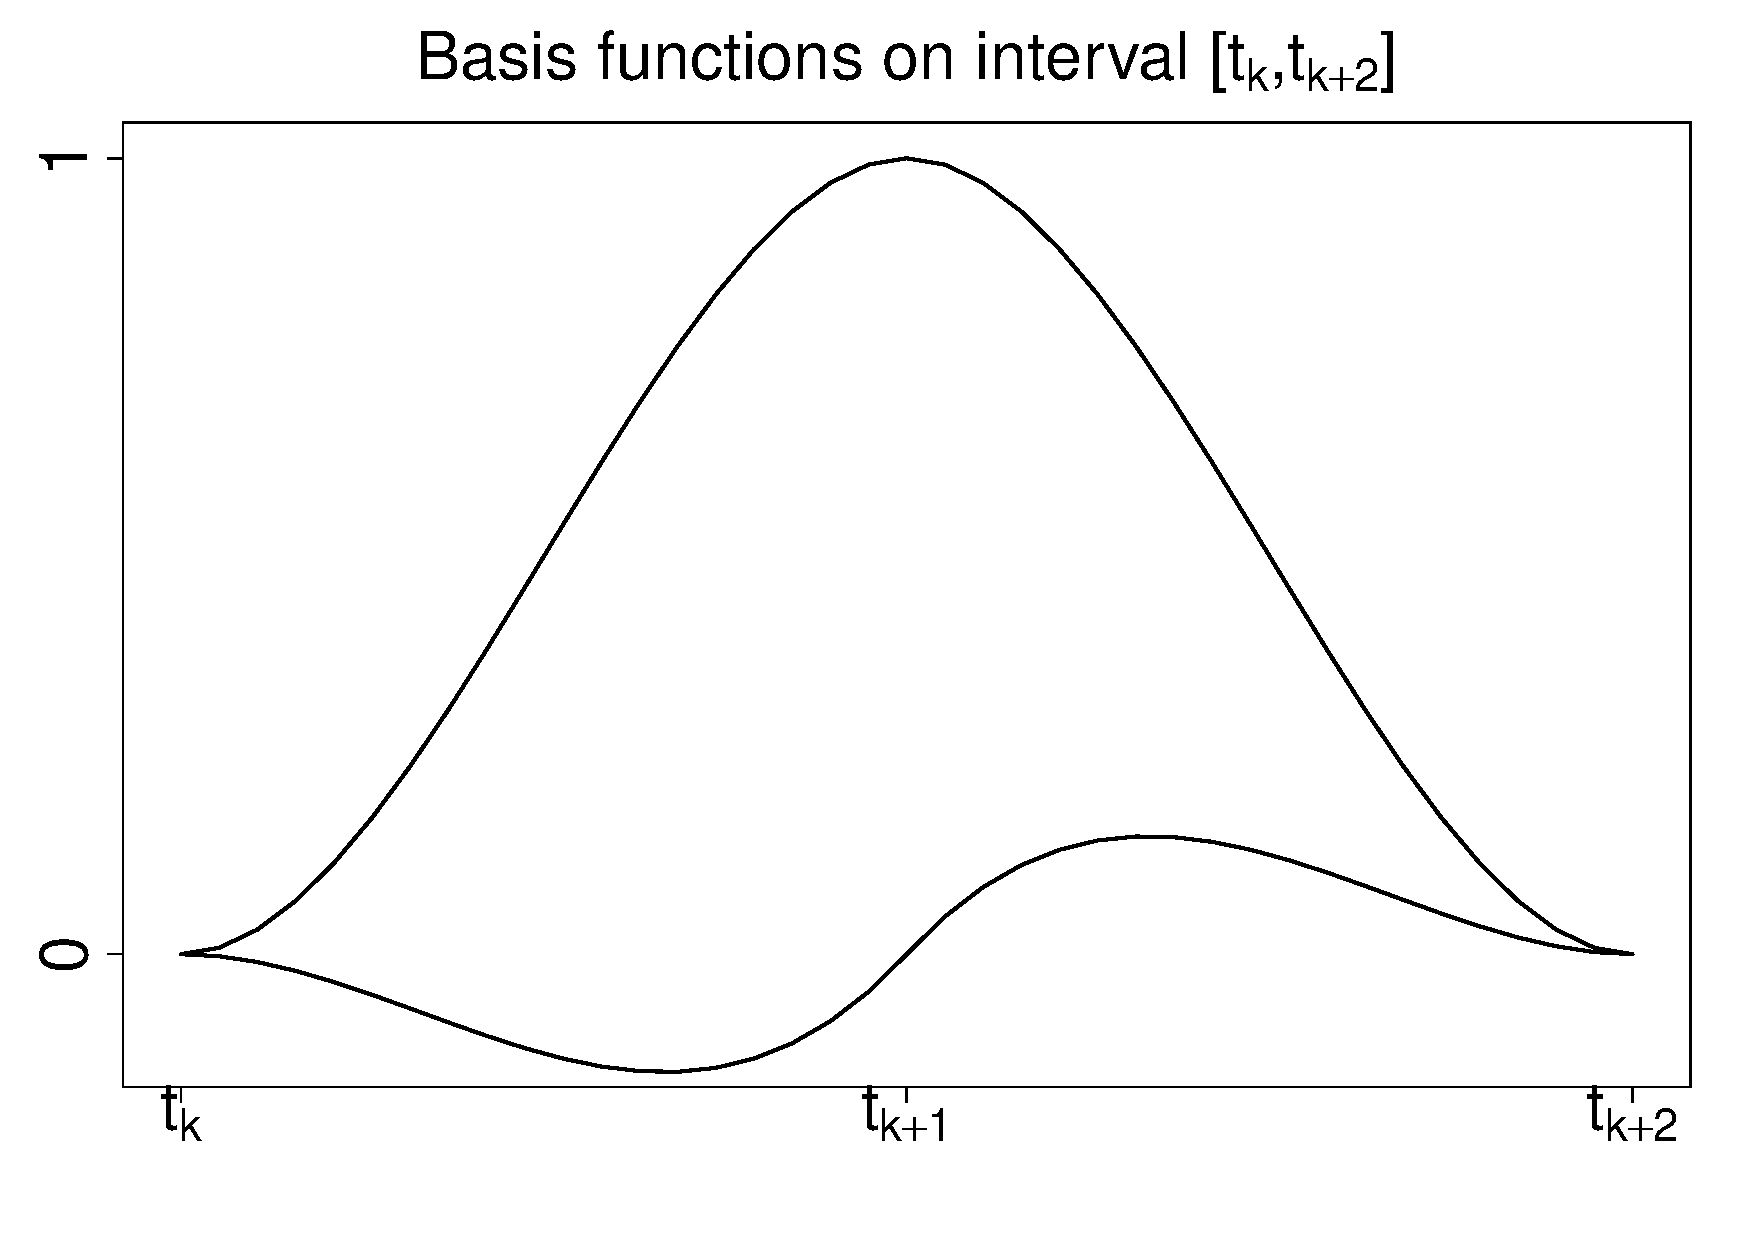
\includegraphics[width=8cm, height=4cm]{Chapters/2.TractorSplineTheory/plot/basistk}
%\small 
\caption{The two basis functions $N_{2k+1}$ and $N_{2k+2}$ on interval $[t_k, t_{k+2})$. It is apparently that these basis functions are continuous on this interval and have continuous first derivatives.}
\label{basisfigure}
\end{figure}



%From the definition of tractor basis functions, it can be seen that at joint knot of two neighbor intervals, Hermite spline basis share the same $y_i$ and $v_i$. With this property, we construct tractor spline basis functions. There are 2 parameters on each joint knots and 4 on the start and end knots. Then the degrees of freedom of parameters should be $2n-4+4=2n$. However $2(n-2)$ constraints are added on the joint knots, that make the spline have continuous first and second derivatives. 2 constraints are added on the start and end knots to keep their first derivatives are continuous. Then the degrees of freedom of parameters is 2. 


\subsection{Solution to The Objective Function}

Basis functions have been defined in the previous subsection, therefore the tractor spline $f(t)$ on $[a,b]$, where $a \leq t_1 < t_2< \cdots < t_{n-1}<t_n \leq b$, can be found by minimizing  objective function (\ref{of2d}), which reduces to
\begin{equation}\label{tractormse}
\text{MSE}(\theta, \lambda,\gamma) = (\mathbf{y}-\mathbf{B}\theta)^\top (\mathbf{y}-\mathbf{B}\theta) +\gamma (\mathbf{v}-\mathbf{C}\theta)^\top (\mathbf{v}-\mathbf{C}\theta)+n \theta^\top\Omega_{\lambda}\theta,
\end{equation}
where $\{\mathbf{B}\}_{ij} = N_j(t_i)$ , $\{\mathbf{C}\}_{ij} = N'_j(t_i)$ and $\{\Omega_{2n}^{(k)} \}_{jk}=\int_{t_k}^{t_{k+1}}\lambda_k N''_j(t)N''_k(t)dt$. After substituting the series observation $t_1, \cdots, t_n$ into basis functions, we get $N_1(t_1)=1, N_1(t_2)=0, \cdots, N_{2k-1}(t_{k})=1, N_{2k}(t_{k})=0, \cdots, N_{2n-1}(t_n)=1, N_{2n}(t_n)=0$; and into first derivative of basis functions, we get $N'_1(t_1)=0, N_1'(t_2)=1, \cdots, N_{2k-1}'(t_{k})=0, N_{2k}'(t_{k})=1, \cdots, N_{2n-1}'(t_n)=0, N_{2n}'(t_n)=1$. That means the matrices $\mathbf{B}$ and $\mathbf{C}$ in MSE equation (\ref{tractormse}) are $n \times 2n$ dimensional and the elements are
\begin{align}
\mathbf{B}&=\{B\}_{ij}=\begin{cases}
1, & j=2i-1\\
0, & \mbox{otherwise}
\end{cases}\\
\mathbf{C}&=\{C\}_{ij}=\begin{cases}
1, & j=2i\\
0, & \mbox{otherwise}
\end{cases}
\end{align}
where $i=1, \cdots, n$.  The $k$-th $\Omega_{\lambda_k}^{(k)}$ is a $2n \times 2n$ matrix and its details is in appendix. Then the penalty term is
\begin{equation}
\mathbf{\Omega}_\lambda=\sum_{k=1}^{n-1}\Omega_{\lambda_k}^{(k)},
\end{equation}
which is a bandwidth four matrix.


The solution to (\ref{tractormse}) is easily seen to be
\begin{equation}\label{thetahat}
\hat{\theta}=(\mathbf{B}^\top\mathbf{B}+\gamma\mathbf{C}^\top\mathbf{C}+n\Omega_{\lambda})^{-1}(\mathbf{B}^\top\mathbf{y}+\gamma\mathbf{C}^\top\mathbf{v})
\end{equation}
a generalized ridge regression. Then the fitted smoothing spline is given by
\begin{equation}
\hat{f}(t)=\sum_{i=1}^{2n}N_i(t)\hat{\theta}_i
\end{equation}

A smoothing spline with parameters $\lambda(t)$ and $\gamma$ is an example of a linear smoother \cite{esl2009}. This is because the estimated parameters in equation (\ref{thetahat}) are a linear combination of $y_i$ and $v_i$. Denote by $\hat{\mathbf{f}}$ and $\hat{\mathbf{f}'}$ the $2n$ vector of fitted values $\hat{f}(t_i)$ and $\hat{f'}(t_i)$ at the training points $t_i$. Then
\begin{equation}
\begin{split}
\hat{\mathbf{f}} =\mathbf{B}(\mathbf{B}^\top\mathbf{B}+\gamma\mathbf{C}^\top\mathbf{C}+n\Omega_{\lambda})^{-1}(\mathbf{B}^\top\mathbf{y}+\gamma\mathbf{C}^\top\mathbf{v})\\
\triangleq \mathbf{S}_{\lambda,\gamma}\mathbf{y}+\gamma\mathbf{T}_{\lambda,\gamma}\mathbf{v} 
\end{split}
\end{equation}
\begin{equation}
\begin{split}
\hat{\mathbf{f}'}
=\mathbf{C}(\mathbf{B}^\top\mathbf{B}+\gamma\mathbf{C}^\top\mathbf{C}+n\Omega_{\lambda})^{-1}(\mathbf{B}^\top\mathbf{y}+\gamma\mathbf{C}^\top\mathbf{v})\\
\triangleq\mathbf{U}_{\lambda,\gamma}\mathbf{y}+\gamma\mathbf{V}_{\lambda,\gamma}\mathbf{v}
\end{split}
\end{equation}
The fitted $\hat{\mathbf{f}}$ and $\hat{\mathbf{f}'}$ are linear in $\mathbf{y}$ and $\mathbf{v}$, and the finite linear operators $\mathbf{S}_{\lambda,\gamma}, \mathbf{T}_{\lambda,\gamma}, \mathbf{U}_{\lambda,\gamma}$ and $\mathbf{V}_{\lambda,\gamma}$ are known as the smoother matrices. One consequence of this linearity is that the recipe for producing $\hat{\mathbf{f}}$ and $\hat{\mathbf{f}'}$ from $\mathbf{y}$ and $\mathbf{v}$, do not depend on $\mathbf{y}$ and $\mathbf{v}$ themselves; $\mathbf{S}_{\lambda,\gamma}, \mathbf{T}_{\lambda,\gamma}, \mathbf{U}_{\lambda,\gamma}$ and $\mathbf{V}_{\lambda,\gamma}$ depend only on $t_i,\lambda(t)$ and $\gamma$.

Suppose in a traditional least squares fitting, $\mathbf{B}_\xi$ is $N \times M$ matrix of $M$ cubic-spline basis functions evaluated at the $N$ training points $x_i$, with knot sequence $\xi$ and $M \ll N$. Then the vector of fitted spline values is given by
\begin{align}\label{fhy}
\hat{\mathbf{f}}=\mathbf{B}_\xi(\mathbf{B}^\top_\xi\mathbf{B}_\xi)^{-1}\mathbf{B}_\xi\mathbf{y}=\mathbf{H}_\xi\mathbf{y}
\end{align}
Here the linear operator $\mathbf{H}_\xi$ is a symmetric, positive semidefinite matrices, and $\mathbf{H}_\xi\mathbf{H}_\xi=\mathbf{H}_\xi$ (idempotent) \cite{esl2009}. In our case, it is easily seen that $\mathbf{S}_{\lambda,\gamma}, \mathbf{T}_{\lambda,\gamma}, \mathbf{U}_{\lambda,\gamma}$ and $\mathbf{V}_{\lambda,\gamma}$ are symmetric, positive semidefinite matrices as well. Additionally, by Cholesky decomposition
\begin{equation}
(\mathbf{B}^\top\mathbf{B}+\gamma\mathbf{C}^\top\mathbf{C}+n\Omega_{\lambda})^{-1}=\mathbf{R}\mathbf{R}^\top,
\end{equation}
it is easily to prove that $\mathbf{T}_{\lambda,\gamma}=\mathbf{B}\mathbf{R}\mathbf{R}^\top\mathbf{C}^\top$ and $\mathbf{U}_{\lambda,\gamma}=\mathbf{C}\mathbf{R}\mathbf{R}^\top\mathbf{B}^\top$, then we will have 
 $\mathbf{T}_{\lambda,\gamma}= \mathbf{U}_{\lambda,\gamma}^\top$. When $\lambda=\gamma=0$, the matrix $\mathbf{S}_{\lambda_0,\gamma_0}=\mathbf{B}(\mathbf{B}^\top\mathbf{B})^{-1}\mathbf{B}^\top$ is idempotent.  

Additionally, by playing with $\lambda(t)$ and $\gamma$, tractor spline has the following property:
\begin{itemize}
\item if $\lambda(t)$ is a piecewise constant and $\gamma \neq 0$, then $f$ and $f'$ are continuous, $f''$ is piecewise linear but not continuous at knots;
\item if $\lambda(t)$ is a piecewise constant and $\gamma = 0$, the same as above;
\item if $\lambda(t)=\lambda $ is a constant and $\gamma \neq 0$, the same as above;
\item if $\lambda(t)=\lambda $ is a constant and $\gamma = 0$, then $f$, $f'$ are continuous, $f''$ is piecewise linear and continuous at knots.
\end{itemize}

%Then we take some sample knots $\mathbf{y}^{(new)}$ with the same size of $\mathbf{y}$ from $\hat{\mathbf{f}}$ and reconstruct the spline function. It is easily seen that
% \begin{equation}
%\hat{\mathbf{f}}^{(new)} = \mathbf{S}_{\lambda_0,\gamma_0}\mathbf{y}^{(new)}=\mathbf{S}_{\lambda_0,\gamma_0}\mathbf{S}_{\lambda_0,\gamma_0}\mathbf{y}=(\mathbf{B}(\mathbf{B}^\top\mathbf{B})^{-1}\mathbf{B}^\top)(\mathbf{B}(\mathbf{B}^\top\mathbf{B})^{-1}\mathbf{B}^\top)=\mathbf{S}_{\lambda_0,\gamma_0}\mathbf{y},
 %\end{equation}
 %which returns the same reconstruction. So $\hat{\mathbf{f}}$ is generated and only affected by $\mathbf{y}$. And the same as $\hat{\mathbf{f}'}$, because
%\begin{equation}
%\hat{\mathbf{f}'}^{(new)}=\mathbf{U}_{\lambda_0,\gamma_0}\mathbf{y}^{(new)}=\mathbf{U}_{\lambda_0,\gamma_0}\mathbf{S}_{\lambda_0,\gamma_0}\mathbf{y}=(\mathbf{C}\mathbf{B} (\mathbf{B}^\top\mathbf{B})^{-1}\mathbf{B}^\top)(\mathbf{B}(\mathbf{B}^\top\mathbf{B})^{-1}\mathbf{B}^\top)\mathbf{y}=\mathbf{U}_{\lambda_0,\gamma_0}\mathbf{y}.
%\end{equation}
 %That means no matter how many times we reconstruct tractor spline, once the matrices are fixed and observed knots are given, it will always return the same results when $\lambda=\gamma=0$.

%\begin{theorem}
%For $n\geq 2$, the objective function $J[f]$ in equation (\ref{of2d}) is minimized by a tractor spline.
%\end{theorem}

\subsection{Adjusted Penalty Term and Parameter Function}
To get the reconstructed trajectory in a multi-dimensional space, one can use tractor spline to find the trajectory in each dimensions simultaneously can combine them together at the end. Additionally, sometimes the data is not recorded in equal space. Due to the property of Hermite spline, the combination of multi-dimensional reconstructions and non-equal space data will bring some issues. Imagining this situation that a vehicle is moving along the $x$-axis, its $x$ position changes consequently, but its $y$ position might stay the same. By fitting $\mathbf{x}$ and $\mathbf{u}$ on $x$-axis, the tractor spline $f_x(t)$ will give us a best fit which returns smallest errors to the objective function. While with the same parameter $\lambda(t)$ and $\gamma$, $f_y(t)$ will return a cubic curve. However, it should give us a straight line as we expected. Moreover, in some circumstances, the time mark increases but $\mathbf{f}$ and $\mathbf{f}'$ keep the same, or changes slightly. Facing this situation, the Hermite spline will return a wiggle in one dimension and a curve in two dimensions. To get a reliable reconstruction, we introduce an adjusted term $\frac{(\Delta t_i)^\alpha}{(\Delta d_i)^\beta}$, where $\alpha \ge 0$ and $\beta \ge 0$, to the penalty function $\lambda(t)$, which means that the tractor spline should be penalized by its real difference of $\Delta d_i$ and $\Delta t_i$ between two points $p_i$ and $p_{i+1}$. With this term, when $\mathbf{u}$ goes down or equals to 0, it will make sure that the penalty function will be large enough and return a straight line rather than a curve in each dimension of $x$ and $y$. Because of the unit of the penalty term is $m^2/t^3$, to keep the same scale in the space, $\alpha$ and $\beta$ in the adjusted penalty term are chosen as 3 and 2. Then the final form of the penalty function is
\begin{equation}\label{adjustedpenalty}
\lambda(t)=\begin{cases}
\frac{(\Delta t_i)^3}{(\Delta d_i)^2}\lambda
\end{cases}, t_i\leq t < t_{i+1}.
\end{equation}
Eventually in objective function there is one parameter $\lambda$ controlling the curvature of tractor spline in different status, and another one parameter $\gamma$ controlling the residuals of velocity. 

\section{Parameter Selection and Cross Validation}

The problem of choosing the smoothing parameter is ubiquitous in curve estimation. And there are two different philosophical approaches to this question. The first one is to regard the free choice of smoothing parameter as an advantageous feature of the procedure. The other one is to find the parameter automatically by the data \cite{green1993nonparametric}. We more prefer the latter one, use data to train our model and find the best parameters. The most well known method is cross-validation.


Assuming that the random errors has zero mean, the true regression curve $f(t)$ has the property that, if an observation $y$ is taken at a point $t$, the value $f(t)$ is the best predictor of $y$ in terms of returning a small value of $(y-f(t))^2$. 

Now we focus on an observation $y_i$ at point $t_i$ as being a new observation by omitting it from the set of data, which are used to estimate $\hat{f}$. Denote by $\hat{f}^{(-i)}(t,\lambda)$ the estimated function from the remaining data, where $\lambda$ is the smoothing parameter. Then $\hat{f}^{(-i)}(t,\lambda)$ minimizes 
\begin{align}\label{originalcv}
\frac{1}{n}\sum_{j \neq i}(y_j-f(t_j))^2+\lambda \int f''^2dt
\end{align}
 and $\lambda$ can be quantified by cross-validation score function
\begin{align}
\mbox{CV}(\lambda)=\frac{1}{n}\sum_{i=1}^{n}\{y_i-\hat{f}^{(-i)}(t_i,\lambda)\}^2.
\end{align}
The basis idea of cross-validation is to choose the value of $\lambda$ that minimizes $\mbox{CV}(\lambda)$. 

An efficient way to calculate cross validation score is given by \cite{green1993nonparametric}. Through the equation (\ref{fhy}), we know that the value of the smoothing spline $\hat{f}$ depend linearly on the data $y_i$. Define the matrix $A(\lambda)$, which is a map vector of observed values $y_i$ to predicted values $\hat{f}(t_i)$. Then we have
\begin{equation}
\hat{\mathbf{f}}=A(\lambda)\mathbf{y}
\end{equation}
and the following lemma.
\begin{lemma}\label{cvlema}
The cross validation score satisfies
\begin{equation}
\mbox{CV}(\lambda)=\frac{1}{n} \sum_{i=1}^n \left(\frac{y_i-\hat{f}(t_i)}{1-A_{ii}(\lambda)}\right)^2
\end{equation}
where $\hat{f}$ is the spline smoother calculated from the full data set $\{(t_i,y_i)\}$ with smoothing paramter $\lambda$.
\end{lemma}

For a tractor spline and its MSE function, there are two parameters need to be estimated $\lambda$ and $\gamma$. Then the objective function (\ref{originalcv}) becomes
\begin{align}
\frac{1}{n}\sum_{j \neq i}(y_j-f(t_j))^2+\frac{\gamma}{n}\sum_{j \neq i}(v_j-f'(t_j))^2+ \int \lambda(t)f''^2dt,
\end{align}
and the cross-validation score function is
\begin{align}
\mbox{CV}(\lambda,\gamma)=\frac{1}{n}\sum_{i=1}^{n}\{y_i-\hat{f}^{(-i)}(t_i,\lambda,\gamma)\}^2.
\end{align}

For a tractor spline, the parameter $\hat{\theta}=(B^\top B+\gamma C^\top C+n\Omega_\lambda)^{-1}(B^\top\mathbf{y}+\gamma C^\top\mathbf{v})$ gives us
\begin{equation}
\begin{split}
 \hat{\mathbf{f}}&=B\hat{\theta}=B(B^\top B+\gamma C^\top C+n\Omega_\lambda)^{-1}B^\top\mathbf{y}+B(B^\top B+\gamma C^\top C+n\Omega_\lambda)^{-1}C^\top\mathbf{v}\\&=S\mathbf{y}+\gamma T\mathbf{v},
 \end{split}
 \end{equation}
 \begin{equation}
 \begin{split}
\hat{\mathbf{f}}'&=C\hat{\theta}=C(B^\top B+\gamma C^\top C+n\Omega_\lambda)^{-1}B^\top\mathbf{y}+C(B^\top B+\gamma C^\top C+n\Omega_\lambda)^{-1}C^\top\mathbf{v}\\&=U\mathbf{y}+\gamma V\mathbf{v}.
 \end{split}
\end{equation}
From lemma \ref{cvlema}, we can prove the following theorem.
\begin{theorem}\label{cvscore}
The cross validation score of a tractor spline satisfies
\begin{equation}\label{tractorcv}
\mbox{CV}(\lambda,\gamma)=\frac{1}{n}\sum_{i=1}^{n} \left( \frac{\hat{f}(t_i)-y_i+\gamma \frac{T_{ii}}{1-\gamma V_{ii}}(\hat{f}'(t_i)-v_i)}{1-S_{ii}-\gamma\frac{T_{ii}}{1-\gamma V_{ii}}U_{ii}} \right)^2
\end{equation}
where $\hat{f}$ is the tractor spline smoother calculated from the full data set $\{(t_i,y_i,v_i)\}$ with smoothing parameter $\lambda$ and $\gamma$.
\end{theorem}

The proof of Theorem \ref{cvscore} follows immediately from a lemma, and gives an expression for the deleted residuals $y_i-\hat{f}^{(-i)}(t_i)$ and $v_i-\hat{f}'^{(-i)}(t_i)$ in terms of $y_i-\hat{f}(t_i)$ and $v_i-\hat{f}'(t_i)$ respectively. 

\begin{lemma} \label{cvlemma}
For fixed $\lambda,\gamma$ and $i$, denote $\mathbf{f}^{(-i)}$ by the vector with components $f_j^{(-i)}=\hat{f}^{(-i)}(t_j,\lambda,\gamma)$,  $\mathbf{f}'^{(-i)}$ by the vector with components $f_j'^{(-i)}=\hat{f}'^{(-i)}(t_j,\lambda,\gamma)$, and define vectors $\mathbf{y}^*$ and $\mathbf{v}^*$ by 
\begin{align}
\begin{cases}
y_j^*=y_j &j \neq i\\
y_i^*=\hat{f}^{(-i)}(t_i) &\mbox{otherwise}
\end{cases},\\
\begin{cases}
v_j^*=v_j &j \neq i\\
v_i^*=\hat{f}'^{(-i)}(t_i) &\mbox{otherwise}
\end{cases}.
\end{align}
Then
\begin{align}
\mathbf{\hat{f}}^{(-i)}&=S\mathbf{y}^*+\gamma T\mathbf{v}^*\\
\mathbf{\hat{f}}'^{(-i)}&=U\mathbf{y}^*+\gamma V\mathbf{v}^*
\end{align}
\end{lemma}


\section{Simulation} %and Error Analysis}


\subsection{Numerical Examples}

In this section, we examine the visual quality of the proposed method with four functions: Blocks, Bumps, HeaviSine and Doppler, which have been used in \cite{donoho1994ideal}, \cite{donoho1995adapting} and \cite{abramovich1998wavelet} because of their caricature features in imaging, spectroscopy and other scientific signal processing. However it is unfair for tractor spline fitting "jump" position in Blocks and Bumps function, because it fits position and velocity simultaneously and these points imply infinite first derivative in original functions, which are impossible for vehicles or individuals. In terms of this issue, we treat these functions as velocity, and use noise free points to generate accurate position data, then add noises back to them.

For calculating consideration, we use $n=1024$ \cite{nason2010wavelet}. Because all noises are randomly generated, for convenience of reinitialization and repetition of comparing, we set random seed as 2016. The noises are independent Gaussian distribution $\epsilon \sim N(0,1)$ and signal-to-noise ratio (SNR) is 7. These data are treated as velocity (first derivative). By setting initial position $y_0=0$, acceleration $a_0=0$ and using the following formula to calculate position
\begin{equation}
y_{i+1}=y_i+(v_i+v_{i+1})\frac{t_{i+1}-ti}{2},
\end{equation}
we can easily generate position data. Then we add some noises, which are independent Gaussian distribution $\epsilon \sim N(0,1)$ and SNR is 7. For wavelet reconstruction, we use the threshold policy of "$sure$" and "$BayesThresh$" with levels $j=4, \cdots, 9$. Penalized B-spline is added in comparison. For tractor spline we have two parameters  $\lambda$ and $\gamma$. To evaluate the performance of the velocity term in objective function (\ref{of2d}) and the adjusted penalty term in (\ref{adjustedpenalty}), the parameter $\gamma$ is set as 0 in one reconstruction of tractor spline, whose objective function and solution become
\begin{equation}\label{ofgamma0}
J[f]_{\gamma=0}= \frac{1}{n} \sum_{i=1}^{n} (f(t_i)-y_i)^2 +\sum_{i=1}^{n-1} \lambda_i\int_{t_i}^{t_{i+1}} f''(t)^2 dt,
\end{equation}
and
\begin{equation}\label{thetahat0}
\hat{\theta}_{\gamma=0}=(\mathbf{B}^\top\mathbf{B}+n\Omega_{\lambda})^{-1}\mathbf{B}^\top\mathbf{y}
\end{equation}
and the adjusted penalty term in (\ref{adjustedpenalty}) was removed from another reconstruction, noted as "tractor spline without APT". Figure (\ref{num1}) to (\ref{num4}) display the original (velocity), generated position, wavelet with two different threshold methods, P-spline and three kinds of tractor spline fitted functions. The parameters $\lambda$ and $\gamma$ of a tractor spline are automatically selected from formula (\ref{tractorcv}) by $\mathit{optim()}$ function in $R$.



\begin{figure}
  \centering
   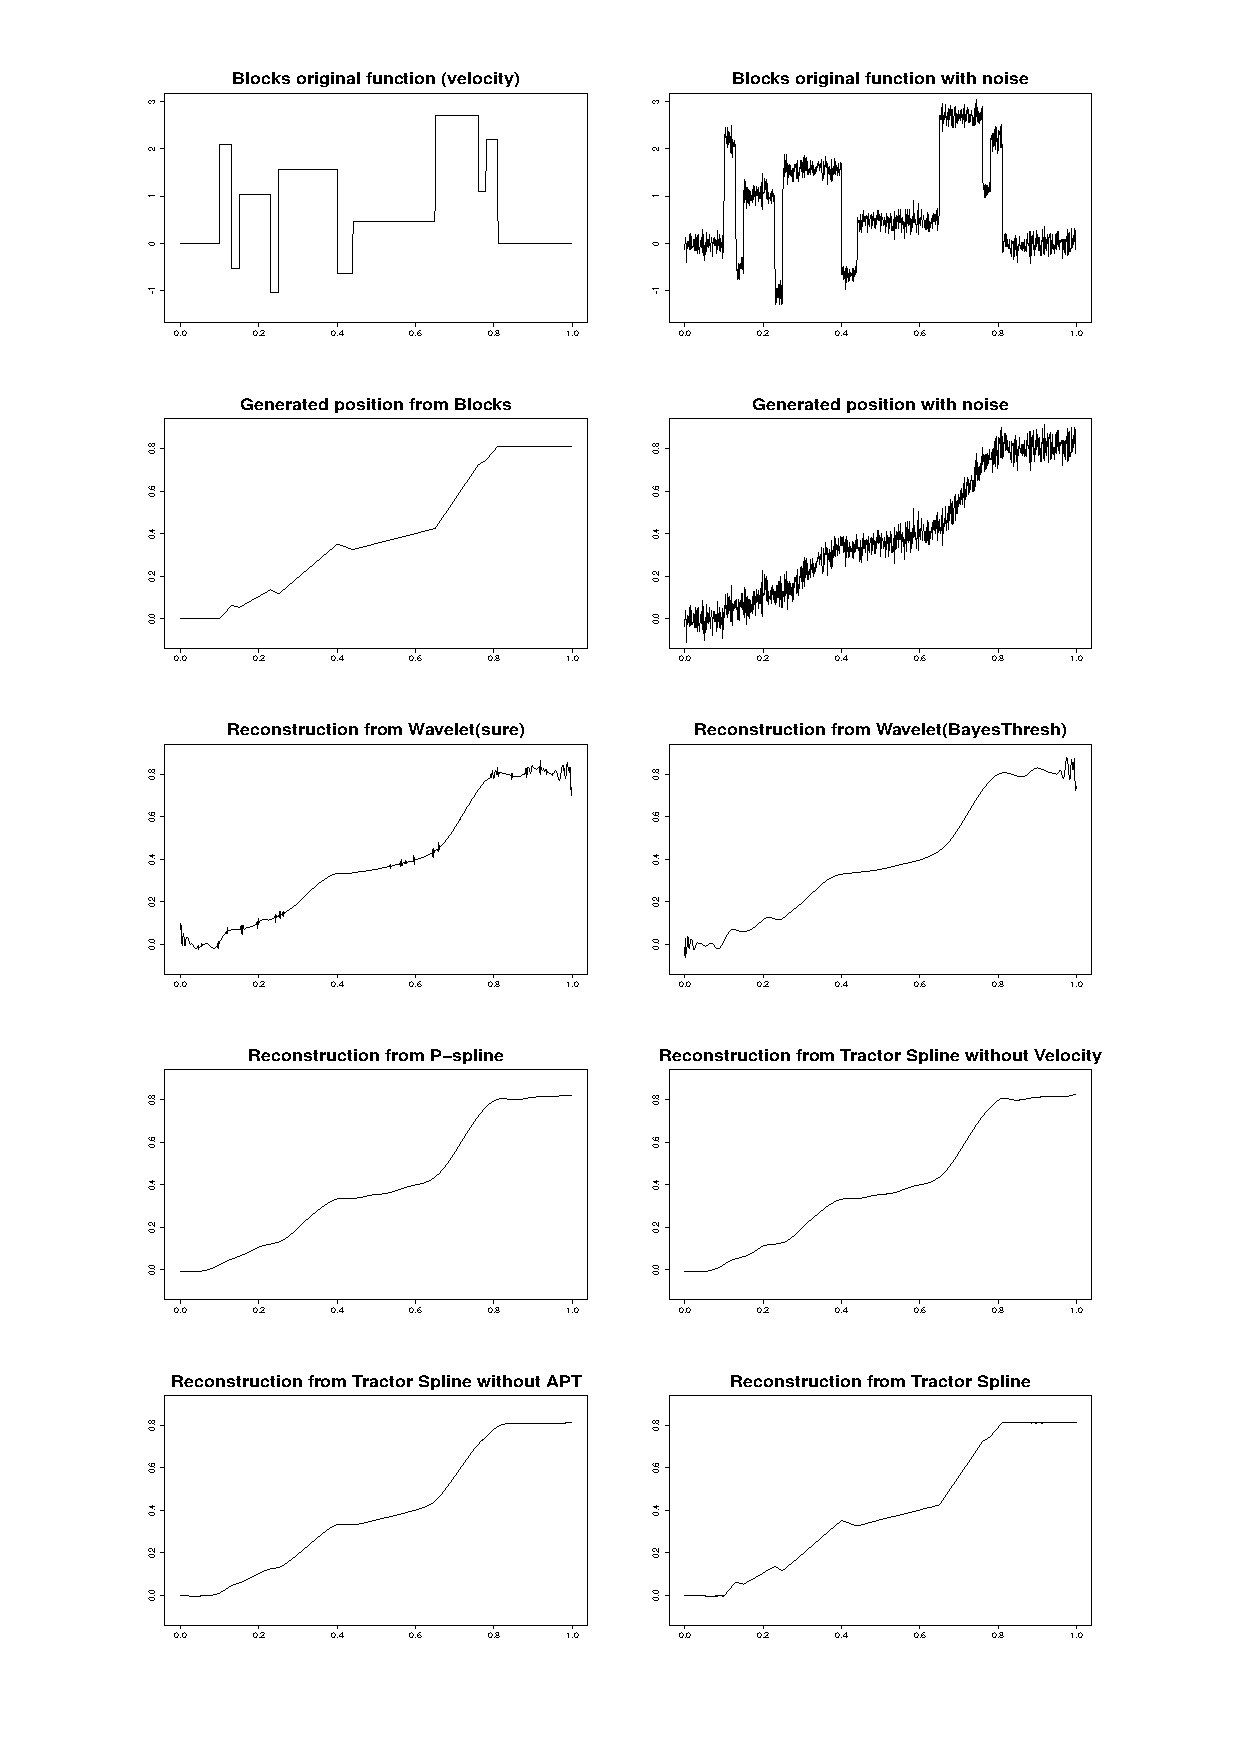
\includegraphics[width=\textwidth,height=14cm]{Chapters/2.TractorSplineTheory/plot/blocks10} 
  \caption{Numerical example: $\textit{Blocks}$. (a) The true velocity function. (b) Velocity with Gaussian noise at SNR=7. (c) Generated position function. (d) Position with Gaussian noise at SNR=7. (e) Reconstruction from Wavelet with sure threshold. (f) Reconstruction from Wavelet with BayesThresh approach. (g) Reconstruction by P-spline. (h) Reconstruction by tractor spline setting $\gamma=0$. (i) Reconstruction by tractor spline with normal penalty term. (j) Reconstruction by proposed tractor spline.}\label{num1}
\end{figure}

\begin{figure}
  \centering
    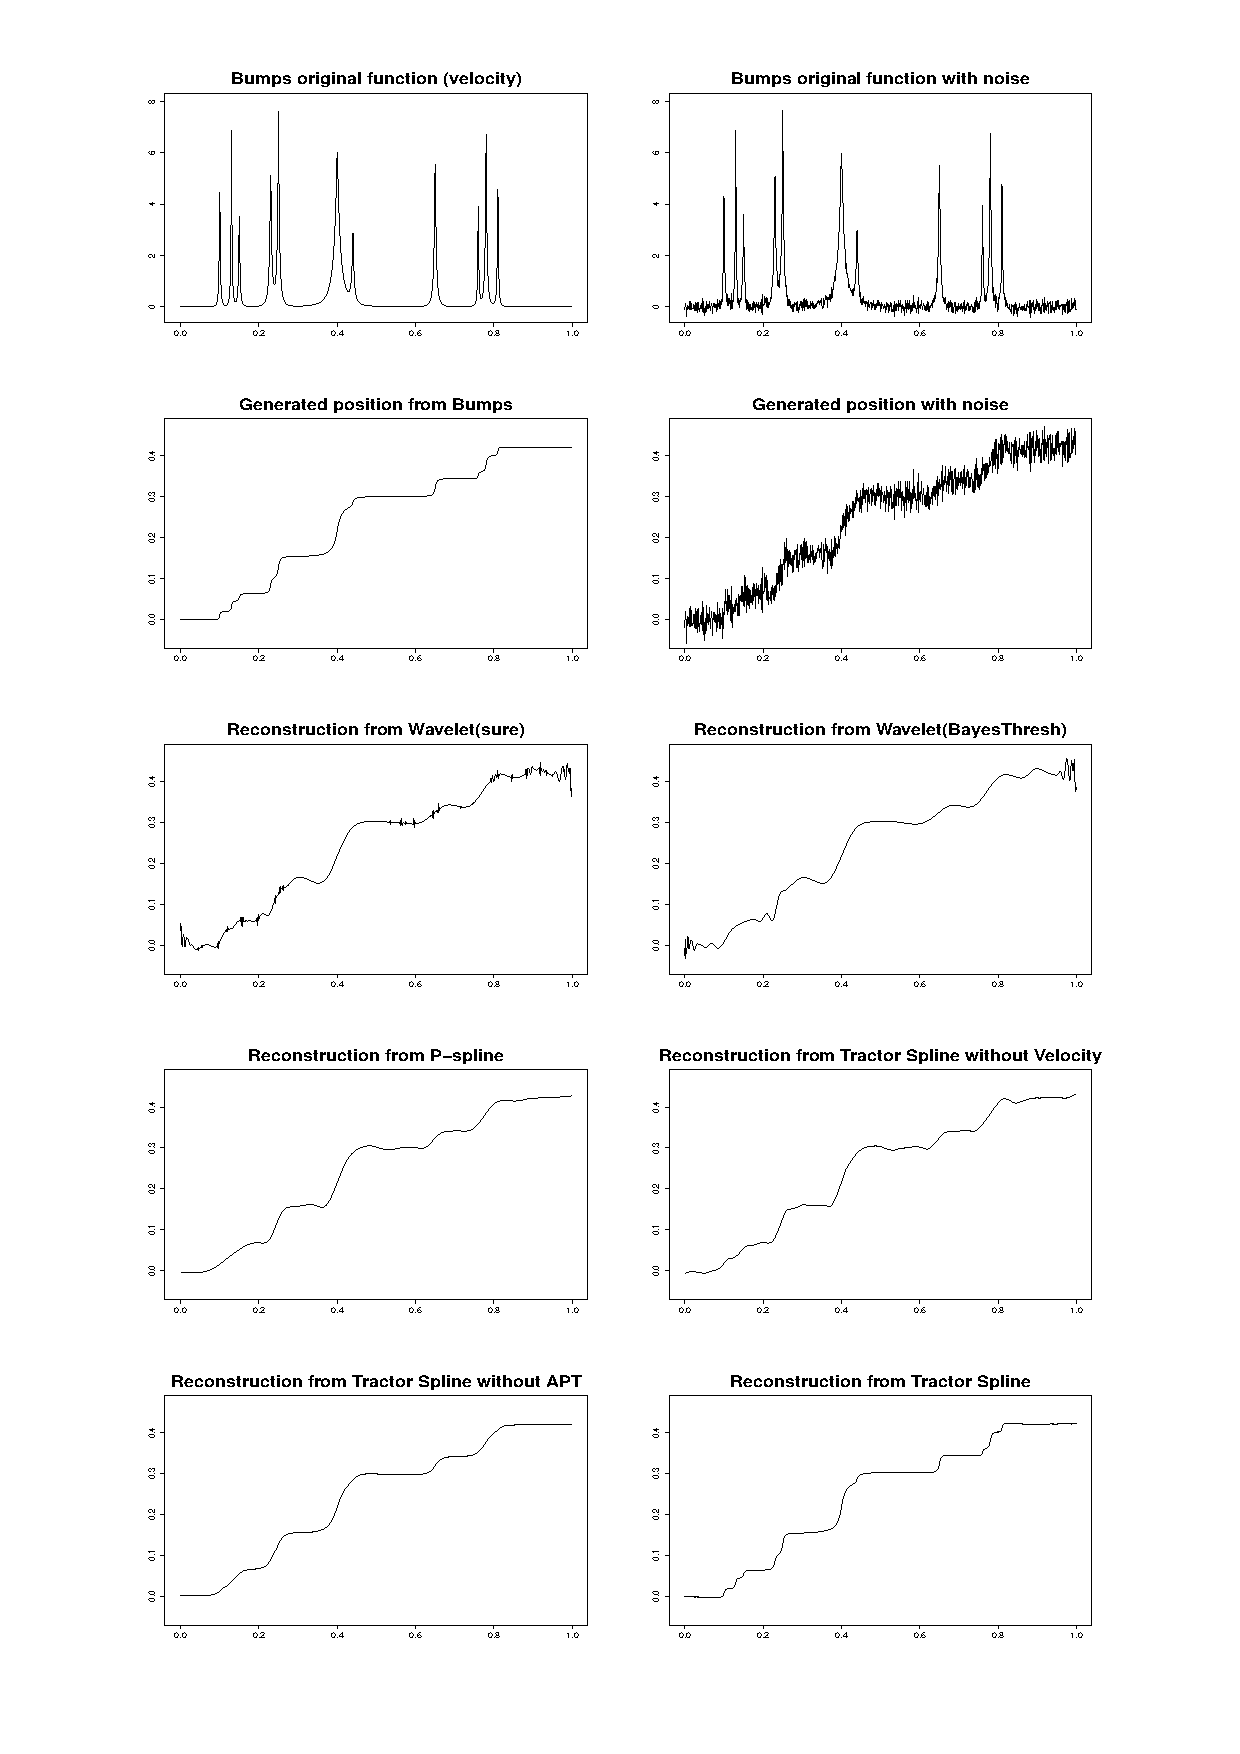
\includegraphics[width=\textwidth,height=14cm]{Chapters/2.TractorSplineTheory/plot/bumps10}
  \caption{Numerical example: $\textit{Bumps}$. (a) The true velocity function. (b) Velocity with Gaussian noise at SNR=7. (c) Generated position function. (d) Position with Gaussian noise at SNR=7. (e) Reconstruction from Wavelet with sure threshold. (f) Reconstruction from Wavelet with BayesThresh approach. (g) Reconstruction by P-spline. (h) Reconstruction by tractor spline setting $\gamma=0$. (i) Reconstruction by tractor spline with normal penalty term. (j) Reconstruction by proposed tractor spline.}\label{num2}
\end{figure}

\begin{figure}
  \centering
    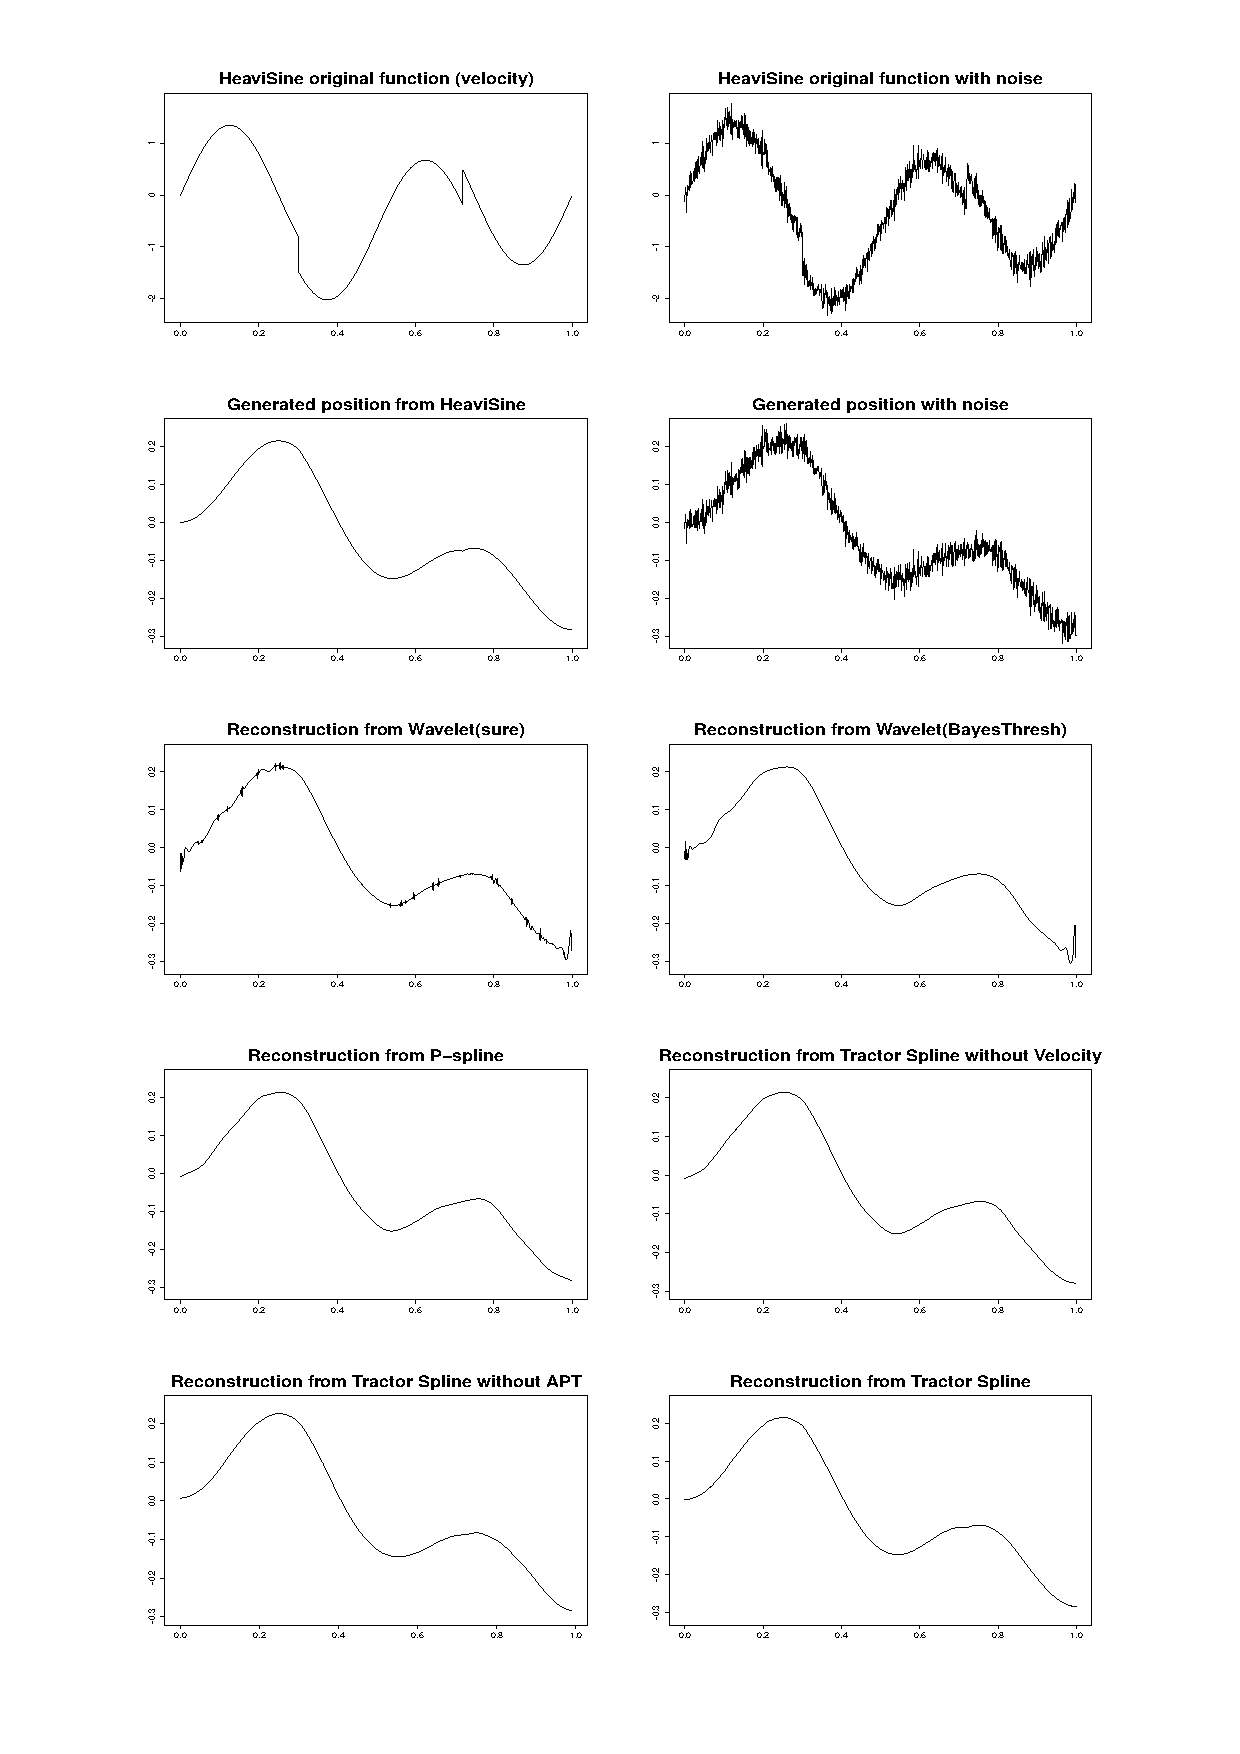
\includegraphics[width=\textwidth,height=14cm]{Chapters/2.TractorSplineTheory/plot/heavi10} 
  \caption{Numerical example: $\textit{HeaviSine}$. (a) The true velocity function. (b) Velocity with Gaussian noise at SNR=7. (c) Generated position function. (d) Position with Gaussian noise at SNR=7. (e) Reconstruction from Wavelet with sure threshold. (f) Reconstruction from Wavelet with BayesThresh approach. (g) Reconstruction by P-spline. (h) Reconstruction by tractor spline setting $\gamma=0$. (i) Reconstruction by tractor spline with normal penalty term. (j) Reconstruction by proposed tractor spline.}\label{num3}
\end{figure}

\begin{figure}
  \centering
         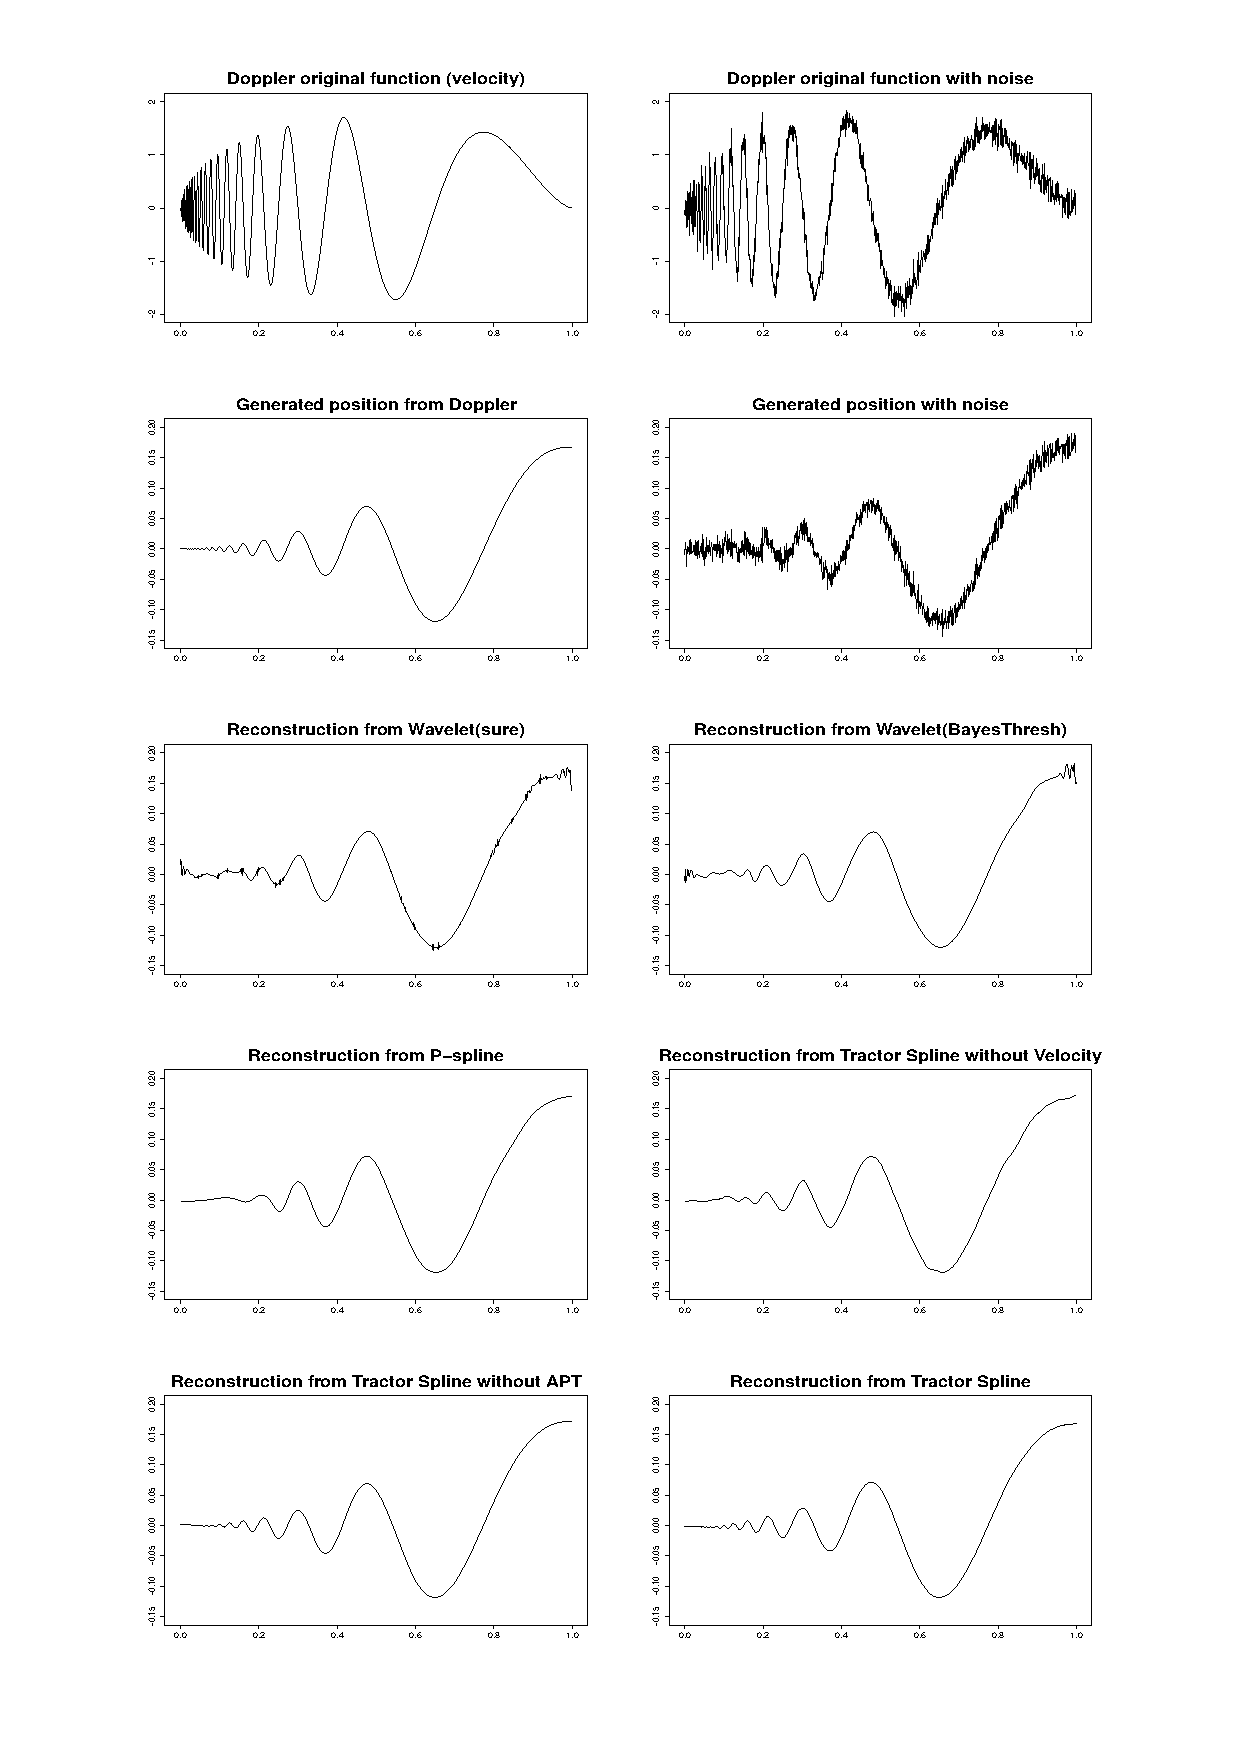
\includegraphics[width=\textwidth,height=14cm]{Chapters/2.TractorSplineTheory/plot/doppler10} 
  \caption{Numerical example: $\textit{Doppler}$. (a) The true velocity function. (b) Velocity with Gaussian noise at SNR=7. (c) Generated position function. (d) Position with Gaussian noise at SNR=7. (e) Reconstruction from Wavelet with sure threshold. (f) Reconstruction from Wavelet with BayesThresh approach. (g) Reconstruction by P-spline. (h) Reconstruction by tractor spline setting $\gamma=0$. (i) Reconstruction by tractor spline with normal penalty term. (j) Reconstruction by proposed tractor spline.}\label{num4}
\end{figure}


By comparing, we can see that all these methods can rebuild up the skeleton of generated trajectory. Wavelets(sure) method have more wiggles in interior interval than Wavelet(BayesThresh), and the latter one becomes fluctuation near boundary knots. P-spline gives much smoother fitting than wavelets, but the drawback is losing more specific details. Tractor spline without velocity might give us less fitting, as can be seen from Blocks and Bumps where there should be a straight line. Tractor spline without adjusted penalty term could also get over fitting when the direction changes more frequently than normal, although it catches specific feature in HeaviSine. The proposed tractor spline performs much better than other methods and returns the near-true trajectory reconstruction.  

Figure \ref{numpenalty} shows the estimated penalty function
\begin{equation}
\lambda(t)=\frac{(\Delta t)^3}{(\Delta d)^2}\lambda.
\end{equation}
The left column illustrates the value of penalty function on different intervals and the right column is the projection on position. Bigger black dots present larger penalty values. It can be seen that $\lambda(t)$ adapts to the smoothness pattern of position and will be large where a long time gap may occur. The details of how this penalty function works will be explained in next subsection.

%and is larger when the function trying to change directions. We only have a couple of large penalty terms in $\mathit{Blocks}$ and $\mathit{Bumps}$ function, as most of the time they were moving in straight line. More curves are in $\mathit{HeaviSine}$ and $\mathit{Doppler}$ functions, so the penalty term try to catch more information and ignore noises. 
\begin{figure}
  \centering
         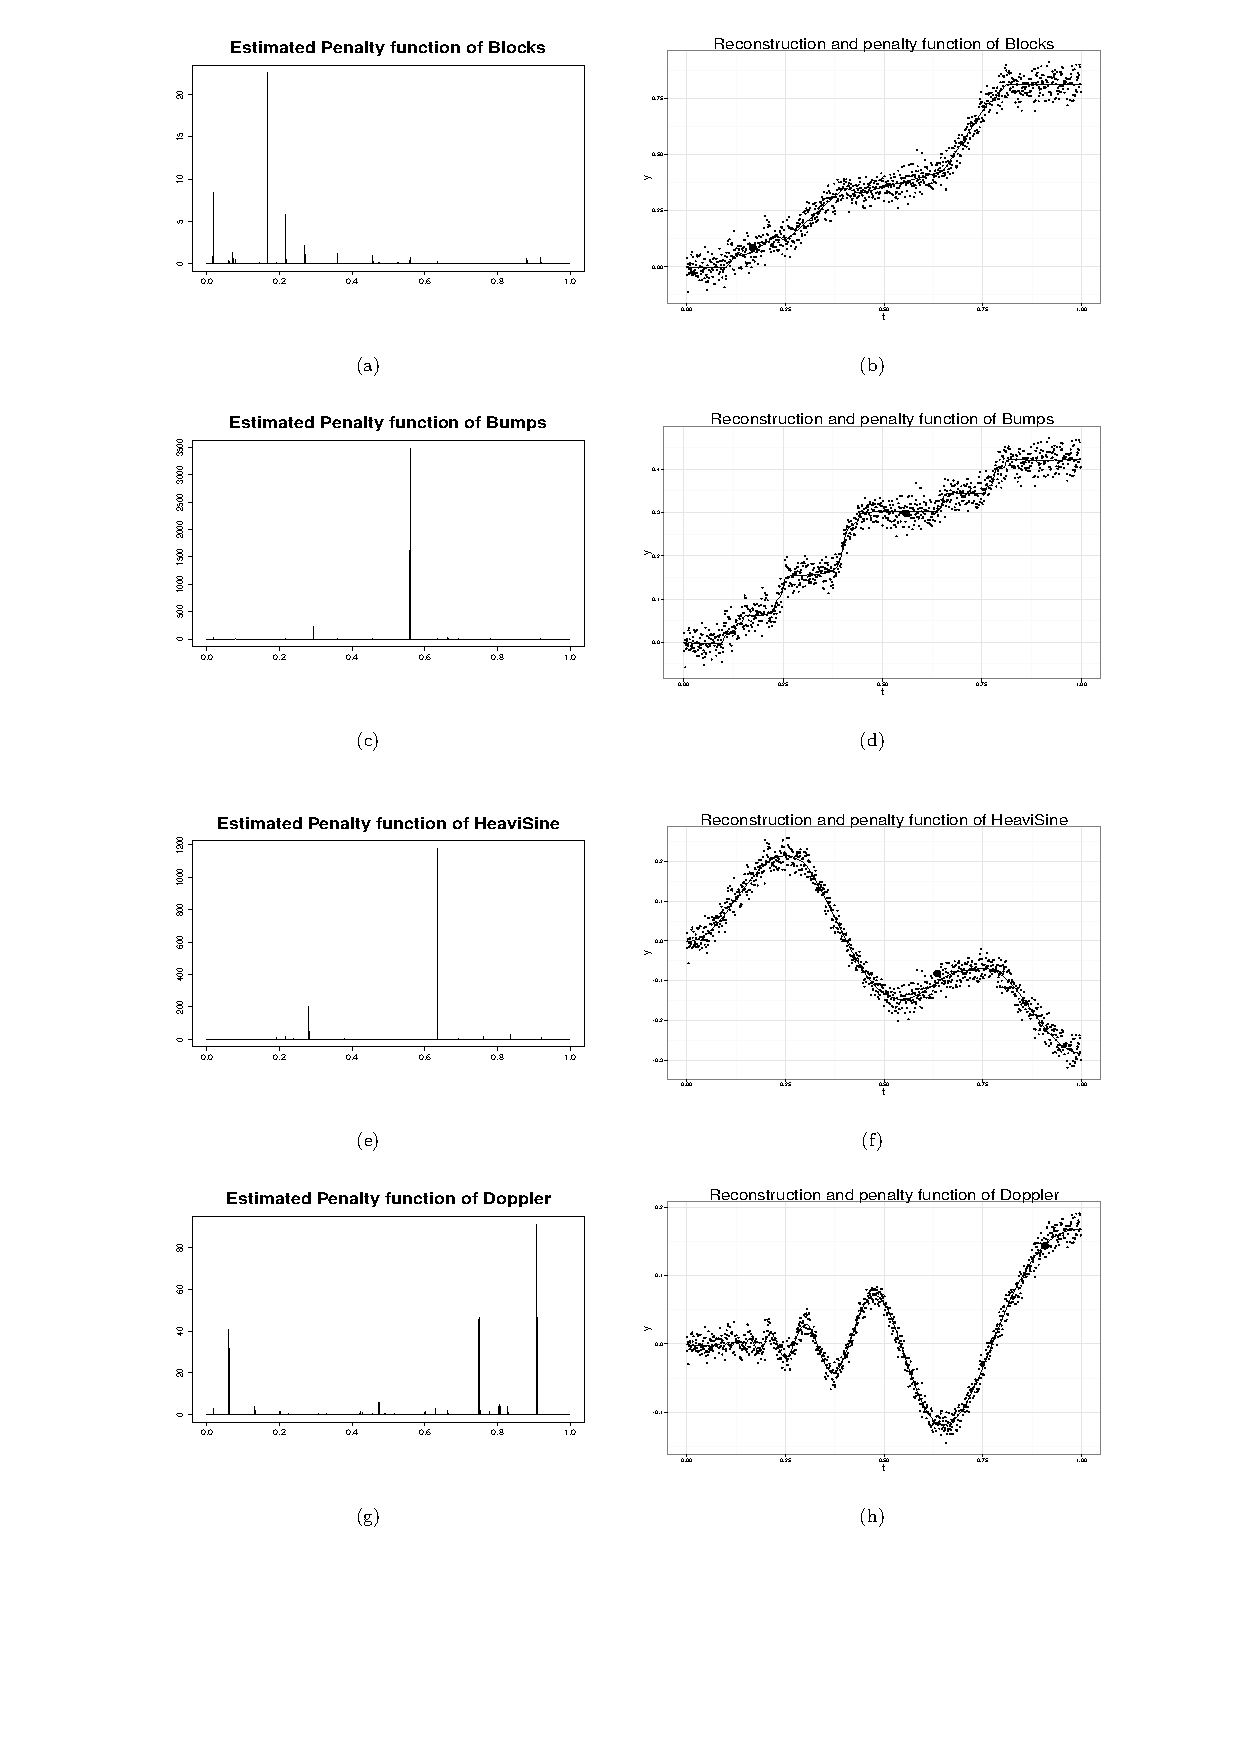
\includegraphics[width=\textwidth,height=14cm]{Chapters/2.TractorSplineTheory/plot/penalty08} 
  \caption{Estimated penalty functions. Left side shows how the value of $\lambda(t)$ changes on the interval. Right side projects $\lambda(t)$ into reconstructions. The bigger the blacks dots present, the larger the penalty values are.}\label{numpenalty}
\end{figure}

Figure \ref{numvtractor} demonstrates the estimated velocity functions. Bt taking the first derivative of fitted tractor spine, it is easily to get the original four velocity functions. The fitting of velocity is not as smooth as that in position, because we only care about the smoothness of position rather than velocity in our cross-validation formula (\ref{cvscore}). However, velocity information dose help us reconstructing trajectory.

\begin{figure}
\centering
%  \begin{landscape}
         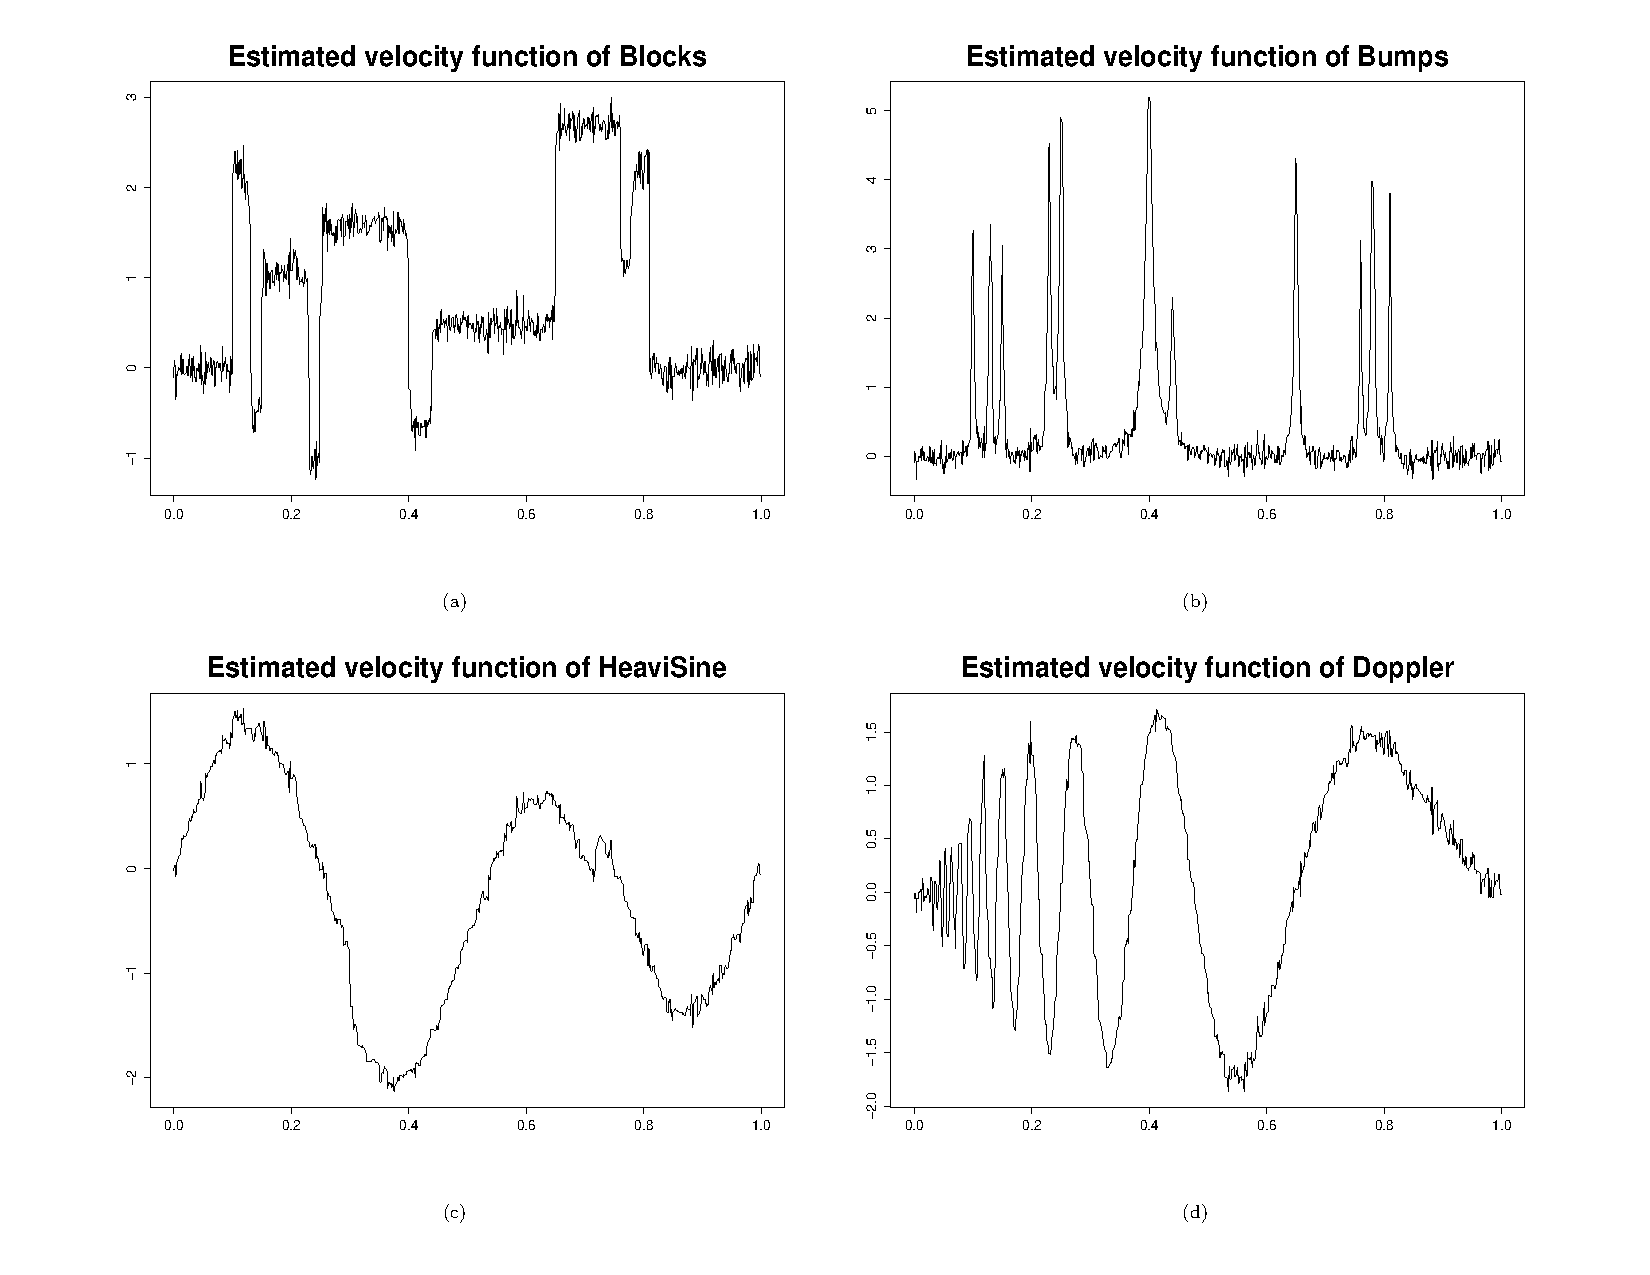
\includegraphics[width=\textwidth,height=9cm]{Chapters/2.TractorSplineTheory/plot/vtractor04} 
%  \end{landscape}
     \caption{Estimated velocity functions by taking the first derivative of tractor spline. (a) Fitted $\mathit{Blocks}$. (b) Fitted $\mathit{Bumps}$. (c) Fitted $\mathit{HeaviSine}$. (d) Fitted $\mathit{Doppler}$.}\label{numvtractor}
\end{figure}


\subsection{Evaluation}
To examine the performance of tractor spline, we conducted a evaluation by comparing the mean square errors and true mean square errors, which are respectively calculated in
\begin{align}
\mbox{MSE}&= \frac{1}{n} \sum_{i=1}^{n} (y_i-\hat{f}_{\lambda,\gamma}(t_i))^2,\\
\mbox{TMSE}&= \frac{1}{n} \sum_{i=1}^{n} (f(t_i)-\hat{f}_{\lambda,\gamma}(t_i))^2.
\end{align}

%Besides the four function in previous subsection, we introduce two more functions as the author did in \cite{liu2010data}: Sin-141 and Sin-1414. The function Sin-141 is divided into three equal length intervals $B_1\oplus B_2 \oplus B_3$ on $[0,1]$ with signal generated by $sin(6\pi t)I\{t\in (B_1,B_3)\} + sin(24\pi t)I(t\in B_2)$, where $I(\cdot)$ is the indicator function. Sin-1414 is divided into four equal length intervals $B_1\oplus B_2 \oplus B_3 \oplus B_4$ on $[0,1]$ with signal generated by $sin(6\pi t)I\{t\in (B_1,B_3)\} + sin(24\pi t)I(t\in B_2,B_4)$

The results are shown in table \ref{mse3200} and \ref{tmse3200}. All of these methods have good performances in fitting noisy data. The differences of mean square error between these methods are not significant, as can be seen from table \ref{mse3200}. The proposed method is not the best among these simulations according to MSE. However, from table \ref{tmse3200}, tractor spline returns the smallest true mean square errors. The difference is significant, that means the reconstruction from tractor spline is closer to the true trajectory. 
 
%\begin{sidewaystable}
 \begin{table}
 	\centering
 	\caption{MSE. Mean square errors of different methods. The star sign (*) marks the smallest error among these methods under the same level. The difference is not significant.}\label{mse3200}
	\setlength\tabcolsep{1.5pt}
	\begin{tabular}{|c|c|r|r|r|r|r|r|}
\hline	MSE ($10^{-4}$)   & SNR & TS & TS$_{\gamma=0}$ & TS$_{APT=0}$  & P-spline & Wavelet(sure)& Wavelet(Bayes)\\ \hline
\textit{Blocks}    & 7   &  16.53& 15.99 & 16.69 & 16.14  & *15.39 & 16.68 \\ \hline
\textit{Blocks}    & 3   &  89.79 & *87.64 & 89.94  & 88.27 & 98.35 & 90.24 \\ \hline
\textit{Bumps}     & 7   & 4.40 & 4.19 & 4.55 & 4.33 & *4.18 & 4.59 \\ \hline
\textit{Bumps}     & 3   & 23.93 & *23.19 & 24.10 & 23.55 & 26.23 & 23.74 \\ \hline
\textit{HeaviSine} & 7   & 4.16 & 4.01 &4.16 & 4.02 & *3.79 & 4.19 \\ \hline
\textit{HeaviSine} & 3   & 22.63 & *22.19 & 22.65 & 22.02 & 23.53 & 22.07 \\ \hline
\textit{Doppler}   & 7   & 1.15 & *1.07 & 1.10 & 1.15  & *1.07 & 1.13  \\ \hline
\textit{Doppler}   & 3   & 6.27 & *5.94 &6.28 & 6.05  & 6.85 & 6.29  \\ \hline
	\end{tabular}
\end{table}
 %\end{sidewaystable}

%\begin{sidewaystable} 
\begin{table}
	\centering
	\caption{TMSE. True mean square errors of different methods. The star sign (*) marks the smallest error among these methods under the same level. The proposed tractor spline returns the smallest TMSE among all the methods under the same level except for $\mathit{Doppler}$ with SNR=7. The differences are significant. }\label{tmse3200}
	\setlength\tabcolsep{1.5pt}
	\begin{tabular}{|c|c|r|r|r|r|r|r|}
\hline	TMSE ($10^{-6}$)  & SNR & TS & TS$_{\gamma=0}$ & TS$_{APT=0}$  & P-spline & Wavelet(sure) & Wavelet(Bayes)\\ \hline
		\textit{Blocks}    & 7   &*1.75 & 54.25 &  28.68   & 54.76   & 201.02   & 182.12   \\ \hline
		\textit{Blocks}    & 3   & *16.44& 152.5 & 30.76  & 171.59   & 1138.08  & 712.36  \\ \hline
		\textit{Bumps}     & 7   &*1.64 & 23.44  & 21.10     & 24.21 & 71.71 & 69.26 \\ \hline
		\textit{Bumps}     & 3   &*8.51 & 77.78  &37.12     & 77.52 & 330.77 & 238.79 \\ \hline
		\textit{HeaviSine} & 7   &*1.53& 7.80  & 1.56     & 9.54   & 55.37  &44.88  \\ \hline
		\textit{HeaviSine} & 3   & *8.21& 33.56  & 8.49 & 34.26 & 240.72& 110.49\\ \hline
		\textit{Doppler}   & 7   & 1.51& 6.67 &  *1.08   &  8.26   & 14.87  & 12.01  \\ \hline
		\textit{Doppler}   & 3   & *8.10& 22.14  & 8.25   & 19.95    &81.48  &50.33   \\ \hline
	\end{tabular}	
\end{table}
%\end{sidewaystable}

\section{Conclusion and Discussion}
%\section{Discussion and Summary}
In this paper, we proposed a tractor spline model with first derivative and adaptive penalty terms to reconstruct trajectory. This method performs better when we know $\mathbf{z}$ and $\mathbf{w}$ information than other methods. Additionally, the reconstruction of a tractor spline contains $4\times (n-1)$ parameters if we have $n$ knots. By adding $2\times (n-2)$ constrains, the original function and its first derivative are continuous on each interior knots, the degrees of freedom will be $4\times (n-1)-2\times (n-2)=2n$. Because there are $n$ location and $n$ velocity data, thus we don't need to specify more parameters or add more constrains on the model. Although the mean square error of tractor spline is not the smallest comparing with other methods, the true mean square error is the smallest most of the time. It means that the reconstruction is closer to the truth. In cross validation, we only focus on the errors of $f$ ignoring that in $f'$. So the reconstruction of $f'$ is not as smooth as that in $f$, which does not affect trajectory reconstruction. A drawback of tractor spline is the cost in finding local minimal parameters, where the cross validation algorithm returns a smaller score. So we optimized our code to make it runs as faster as it can.








\section{Introduction}


\subsection{Spline}

In interpolation and curve fitting, piecewise linear approximation may not have the practical significance of cubic spline, or even higher order, approximation. These "broken lines" are neither very smooth nor very efficient approximation. Researchers can go to piecewise polynomial approximation with higher order pieces \cite{de1978practical}, which is called spline method. A spline is a numeric function that is piecewise-defined by polynomial functions, and which possesses a high degree of smoothness at the places where the polynomial pieces connect (known as knots) \cite{judd1998numerical}\cite{chen2009feedback}. Suppose we are given observed data $t_1,t_2, \cdots, t_n$ on interval $[0,1]$, satisfying $0\leq t_1< t_2 < \cdots <t_n \leq 1$. A piecewise polynomial function $f(t)$ can be obtained by dividing the interval into contiguous intervals $(t_1,t_2),\cdots,(t_{n-1},t_n)$ and represented by a separate polynomial in each interval. For any continuous $f\in \mathbb{C}^{(m)}[0,1]$, it can be represented in a linear combination of basis functions $h_m(t)$, just as every vector in a vector space can be represented as a linear combination of basis vectors. So we have
\begin{equation}\label{fbasis}
f(t) =\sum_{m=1}^{M}\beta_mh_m(t),
\end{equation}
where $\beta_m$ are coefficients \cite{ellis2009}. 

Suppose we were attempt to fit a model of $f(t)$ by least squares without any restrictions, the best fitting $\hat{f}(t)$ would go through every given data to reduce sum of squares to zero. Most of the time, the results are unsatisfactory as explanations of the given data. The roughness penalty approach is introduced to quantify the notion of a rapidly fluctuating curve and then to pose the estimation problem in a way that makes explicit the necessary compromise between varying rapidly fluctuation and slowly trend in curve estimation \cite{green1993nonparametric}. By adding a penalty term $\int_{0}^{1}(f^{(m)}(t))^2dt$, the curve estimate $\hat{f}(t)$ exists and is unique over all spline functions $f(t)$ with $m-1$ continuous derivatives fitting observed data in the space $\mathbb{C}^{(m)}[0,1]$, and it can be found by minimizing the following penalized mean residual sum  squares
\begin{equation}\label{mse}
\text{MSE}(f,\lambda)=\frac{1}{n}\sum_{i=1}^n(f(t_i)-y_i)^2+\lambda \int_{0}^{1}(f^{(m)}(t))^2dt,
\end{equation}
where $\lambda$ is a fixed smoothing parameter, $(t_i,y_i)$, $i=1, \cdots, n$ are observed data and $0 \leq t_1< t_2 < \cdots <t_n \leq 1$. In equation (\ref{mse}),  the smoothing parameter $\lambda$ controls the trade-off between over-fitting and bias. Smoothing spline provides a powerful tool to estimate nonparametric functions \cite{hastie1990generalized}. 

\subsection{Gaussian Process Regression}

A Gaussian Process is a collection of random variables, any finite number of which have a joint Gaussian distribution \cite{b_gpml}. It is fully defined by its mean $m(t)$ and covariance $K(s,t)$ functions as
\begin{align}
m(t)&=\mathbb{E}[f(t)] \\
K(s,t)&=\mathbb{E}[(f(s)-m(s)) (f(t)-m(t))],
\end{align}
where $s$ and $t$ are two variables, and a function $f$ distributed as such is denoted in form of
\begin{equation}
f \sim GP(m(t),K(s,t)).
\end{equation}
Usually the mean function is assumed to be zero everywhere. 

Given a set of input variables $\mathbf{T}$ for function $f(t)$ and the output $\mathbf{y}=f(\mathbf{T})+\varepsilon$ with independent identically distributed Gaussian noise $\varepsilon$ with variance $\sigma_n^2$,  we can use the above definition to predict the value of the function $f_*=f(t_*)$ at a particular input $t_*$. As the noisy observations becoming
\begin{align}\label{covdef}
\text{cov}(y_p,y_q) = K(t_p,t_q)+\sigma_n^2 \delta_{pq}
\end{align}
where $\delta_{pq}$ is a Kronecker delta which is one iff $p=q$ and zero otherwise, the joint distribution of the observed outputs $\mathbf{y}$ and the estimated output $f_*$ according to prior is
\begin{equation}
\left[ \begin{matrix}
\mathbf{y}\\
f_*
\end{matrix} \right] \sim N \left(  
0,\left[   \begin{matrix}
K(\mathbf{T},\mathbf{T}) +\sigma_n^2I& K(\mathbf{T},t_*) \\
K(t_*,\mathbf{T}) & K(t_*,t_*)
\end{matrix}  \right] 
\right).
\end{equation}
The posterior distribution over the predicted value is obtained by conditioning on the observed data
\begin{equation}
f_* | \mathbf{y},\mathbf{T},t_* \sim N(\bar{f_*},\text{cov}(f_*))
\end{equation}
where 
\begin{align}
\bar{f_*}&=\mathbb{E}[f_* | \mathbf{y},\mathbf{T},t_* ]=K(t_*,\mathbf{T})[K(\mathbf{T},\mathbf{T})+\sigma_n^2I]^{-1}\mathbf{y},\\
\text{cov}(f_*)&=K(t_*,t_*)-K(t_*,\mathbf{T})[K(\mathbf{T},\mathbf{T})+\sigma_n^2I]^{-1}K(\mathbf{T},t_*).
\end{align}

\subsection{The Smoothing Spline as Bayes Estimates}
It is possible to interpret the smoothing spline regression estimator as a Bayesian estimate when the mean function $r( .)$ is given an improper prior distribution. \cite{berlinet2011reproducing}
\cite{wahba1990spline}


Consider the model
\begin{equation}
y_i=f(t_i)+\varepsilon_i, 
\end{equation}
where $i=1, \dots, n$, $\varepsilon_i$ are i.i.d. Gaussian distributed noise with variance $\sigma^2$. Assume $f\in \mathbb{H}^{(m)}[0,1]$, where
\begin{equation}
\mathbb{H}^{(m)}[0,1]=\{f:f^{(\nu)} \mbox{absolutely continuous}, \nu=0,\cdots,m-1, \int_{0}^{1} (f^{(m)}(t)^2dt<\infty \}.
\end{equation}
A smoothing spline $\hat{f}_\lambda$ is the minimizer of objective function (\ref{mse}) \cite{wang1998smoothing}. Equipped with an appropriate inner product
\begin{equation}
\langle f,g\rangle=\sum_{\nu=0}^{m-1}f^{(\nu)}(0)g^{(\nu)}(0)+\int_{0}^{1}f^{(m)}g^{(m)}dt,
\end{equation}
the space $\mathbb{H}^{(m)}[0,1]$ becomes a reproducing kernel Hilbert space.

Let $\phi_\nu (t)=\frac{t^{\nu-1}}{(\nu-1)!}$ where $\nu=1, \cdots, m$ and $R_1(s,t)=\int_0^1\frac{ (s-u)_+^{m-1}}{(m-1)!} \frac{ (t-u)_+^{m-1}}{(m-1)!} du$. Denote $S=\{\phi_\nu (t_i) \}_{n\times m}$ where $i=1, \cdots, n, \nu=1, \cdots, m$ and $Q=\{ R_1(t_i,t_j)\}_{n\times n}$ where $i=1, \cdots, n, j=1, \cdots, n$. \cite{kimeldorf1971some} and \cite{kimeldorf1970correspondence}  proved that $\hat{f}_\lambda$ has the form
\begin{equation}
\hat{f}(t)=\sum_{\nu=1}^m d_\nu \phi_\nu(t)+\sum_{i=1}^n c_iR_1(t,t_i).
\end{equation}
By denoting $M=Q+n\lambda I$, \cite{gubook} found that the coefficients will be given by
\begin{align}
\mathbf{c}&=(M^{-1}-M^{-1}S(S^\top M^{-1}S)^{-1}S^\top M^{-1})\mathbf{Y},\\
\mathbf{d}&=(S^\top M^{-1}S)^{-1}S^\top M^{-1}\mathbf{Y}.
\end{align}


\section{Tractor Spline}

A tractor spline $f$ is the solution to the following objective function
\begin{equation}\label{mse2}
\text{MSE}(f,\lambda,\gamma)=\frac{1}{n}\sum_{i=1}^n(f(t_i)-y_i)^2+\frac{\gamma}{n} \sum_{i=1}^n(f'(t_i)-v_i)^2+\int_{0}^{1}\lambda (t)(f^{(m)}(t))^2dt.
\end{equation}
Velocity information is incorporated into MSE in equation (\ref{mse}) by the addition of velocity term $(f'(t_i)-v_i)^2$. The velocity data set $v_i$ are used to estimate $f(t)$ with location data $y_i$ simultaneously. As $f$ is a linear combination of basis functions shown in (\ref{fbasis}), so $f'$ is a linear combination of the first derivative of these basis functions
\begin{equation}
f'(t) =\sum_{m=1}^{M}\alpha_mh'_m(t).
\end{equation}

In the model $y=f(t)+\varepsilon$, it is reasonable to assume that the observed data $y_i$ is Gaussian distributed with mean $f(t_i)$ and variance $\sigma_n^2$. In a similar way, the velocity is estimated as  $v=f'(t)+\frac{\varepsilon}{\gamma}$, where $v_i$ is Gaussian distribution with mean $f'(t_i)$ and variance $\frac{\sigma_n^2}{\gamma}$. Then the joint distribution of $\mathbf{y},\mathbf{v},f(t)$ and $f'(t)$ is normal with zero mean and a covariance matrix, which can be estimated through Gaussian Process Regression.

Suppose we have observed dataset $t_1<t_2<\cdots<t_n$. The function $f(t)$ defined on this interval $[t_1,t_n]$ is called tractor spline, if on each interval $(t_i,t_{i+1})$, $i=2,\cdots,n-2$, $f(t)$ is a cubic polynomial, but on interval $(t_1,t_2)$ and $(t_{n-1},t_n)$ can be a linear function; $f(t)$ fits together at each point $t_i$ in such a way that $f(t)$ itself and its first and second derivatives are continuous at each $t_i$,  $i=2,\cdots,n-2$.  

On an arbitrary interval $[t_i,t_{i+1}]$, we have Hermite Spline basis functions as following
\begin{align}\label{hermitebasis1}
&h_{00}^{(i)}(t)=
\begin{cases}
2(\frac{t-t_{i}}{t_{i+1}-t_{i}})^3-3(\frac{t-t_{i}}{t_{i+1}-t_{i}})^2+1 & t_i\leq t<t_{i+1} \\ 
0 & \mbox{otherwise}
\end{cases}, \\
&h_{10}^{(i)}(t)=\begin{cases}
\frac{(t-t_{i})^3}{(t_{i+1}-t_{i})^2}-2\frac{(t-t_{i})^2}{t_{i+1}-t_{i}}+(t-t_{i}) & t_i\leq t<t_{i+1} \\ 
0 &   \mbox{otherwise}
\end{cases},\\
&h_{01}^{(i)}(t)=
\begin{cases}
-2(\frac{t-t_i}{t_{i+1}-t_i})^3+3(\frac{t-t_i}{t_{i+1}-t_i})^2 & t_i\leq t<t_{i+1} \\ 
0 &   \mbox{otherwise}
\end{cases},\\
&h_{11}^{(i)}(t)=\begin{cases}
\frac{(t-t_i)^3}{(t_{i+1}-t_i)^2}-\frac{(t-t_i)^2}{t_{i+1}-t_i} & t_i\leq t<t_{i+1} \\ 
0 &   \mbox{otherwise}
\end{cases}.
\end{align}

Then a Hermite spline $f^{(i)}(t)$ on interval $[t_i,t_{i+1})$ with points $p_i=\{y_i,v_i\}$ and $p_{i+1}=\{y_{i+1},v_{i+1} \}$  can be expressed as
\begin{equation}
f^{(i)}(t)=h_{00}^{(i)}(t)y_i+h_{10}^{(i)}(t)v_i+h_{01}^{(i)}(t)y_{i+1}+h_{11}^{(i)}(t)v_{i+1}.
\end{equation}

To construct a tractor spline on the entire interval $[t_1,t_n]$, the new basis functions are defined in such way, that $N_1 = h^{(1)}_{00}$, $N_2 = h^{(1)}_{10}$, and for all $k=1,2,\ldots,n-2$, 
\begin{align}
N_{2k+1}&=
\begin{cases}
h_{01}^{(k)}+h_{00}^{(k+1)} & \mbox{if $t<t_n$}\\
2(\frac{t-t_{n-1}}{t_{n}-t_{n-1}})^3-3(\frac{t-t_{n-1}}{t_{n}-t_{n-1s}})^2+1 &  \mbox{if $t=t_n$}
\end{cases},\\
N_{2k+2}&=
\begin{cases}
h_{11}^{(k)}+h_{10}^{(k+1)} & \mbox{if $t<t_n$}\\
\frac{(t-t_{n-1})^3}{(t_{n}-t_{n-1})^2}-2\frac{(t-t_{n-1})^2}{t_{n}-t_{n-1}}+(t-t_{n-1}) & \mbox{if $t=t_n$}
\end{cases},
\end{align}
and
\begin{align}
N_{2n-1} &= 
\begin{cases}
h_{01}^{(n-1)} & \mbox{if $t<t_n$}\\ 
-2(\frac{t-t_{n-1}}{t_{n}-t_{n-1}})^3+3(\frac{t-t_{n-1}}{t_{n}-t_{n-1}})^2 & \mbox{if $t=t_n$}
\end{cases},\\
N_{2n} &= 
\begin{cases}
h_{11}^{(n-1)} & \mbox{if $t<t_n$}\\
\frac{(t-t_{n-1})^3}{(t_{n}-t_{n-1})^2}-\frac{(t-t_{n-1})^2}{t_{n}-t_{n-1}} & \mbox{if $t=t_n$}
\end{cases}.
\end{align}



As independent basis functions, $N_1(t), \cdots, N_{2n}(t)$ span a $2n$ dimensional space $\mathbb{H}$. For any $f \in \mathbb{H}$, it is represented in the form of
\begin{equation}
f=\sum_{i=1}^{2n} \theta_i N_i(t).
\end{equation}

Suppose that we have observations $y_1,\cdots,y_n$ and $v_1,\cdots,v_n$. $f(t)$ can be found by minimizing equation (\ref{mse2}), which reduces to
\begin{equation}\label{tractormse}
\text{MSE}(\theta, \lambda,\gamma) = (\mathbf{y}-\mathbf{B}\theta)^\top (\mathbf{y}-\mathbf{B}\theta) +\gamma (\mathbf{v}-\mathbf{C}\theta)^\top (\mathbf{v}-\mathbf{C}\theta)+n\lambda \theta^\top\Omega\theta
\end{equation}
where $\{\mathbf{B}\}_{ij} = N_j(t_i)$ , $\{\mathbf{C}\}_{ij} = N'_j(t_i)$ and $\{\Omega_{2n} \}_{jk}=\int N''_j(t)N''_k(t)dt$. After substituting the series observation $t_1, \cdots, t_n$ into basis functions, we get $N_1(t_1)=1, N_1(t_2)=0, \cdots, N_{2k-1}(t_{k})=1, N_{2k}(t_{k})=0, \cdots, N_{2n-1}(t_n)=1, N_{2n}(t_n)=0$; and into first derivative of basis functions, we get $N'_1(t_1)=0, N_1'(t_2)=1, \cdots, N_{2k-1}'(t_{k})=0, N_{2k}'(t_{k})=1, \cdots, N_{2n-1}'(t_n)=0, N_{2n}'(t_n)=1$. That means the matrices $\mathbf{B}$ and $\mathbf{C}$ in MSE equation (\ref{tractormse}) are $n \times 2n$ dimensional and the elements are
\begin{align}
\mathbf{B}&=\{B\}_{ij}=\begin{cases}
1, & j=2i-1\\
0, & otherwise
\end{cases}\\
\mathbf{C}&=\{C\}_{ij}=\begin{cases}
1, & j=2i\\
0, & otherwise
\end{cases}
\end{align}
where $i=1, \cdots, n$.  Elements of penalty matrix $\{\Omega_{2n} \}_{jk}$ is given in appendices. 

The solution to (\ref{tractormse}) is easily seen to be
\begin{equation}\label{thetahat}
\hat{\theta}=(\mathbf{B}^\top\mathbf{B}+\gamma\mathbf{C}^\top\mathbf{C}+n\lambda\Omega)^{-1}(\mathbf{B}^\top\mathbf{y}+\gamma\mathbf{C}^\top\mathbf{v})
\end{equation}
a generalized ridge regression. Then the fitted smoothing spline is given by
\begin{equation}
\hat{f}(t)=\sum_{i=1}^{2n}N_i(t)\hat{\theta}_i
\end{equation}

A smoothing spline with parameters $\lambda$ and $\gamma$ is an example of a linear smoother \cite{esl2009}. This is because the estimated parameters in (\ref{thetahat}) are a linear combination of $y_i$ and $v_i$. Denote by $\hat{\mathbf{f}}$ the $2n$ vector of fitted values $\hat{f}(t_i)$ and $\hat{\mathbf{f}'}$ the $2n$ vector of fitted values $\hat{f'}(t_i)$ at the training points $t_i$. Then
\begin{equation}
\begin{split}
\hat{\mathbf{f}} =\mathbf{B}(\mathbf{B}^\top\mathbf{B}+\gamma\mathbf{C}^\top\mathbf{C}+n\lambda\Omega)^{-1}(\mathbf{B}^\top\mathbf{y}+\gamma\mathbf{C}^\top\mathbf{v})\\
\triangleq \mathbf{S}_{\lambda,\gamma}\mathbf{y}+\gamma\mathbf{T}_{\lambda,\gamma}\mathbf{v} 
\end{split}
\end{equation}
\begin{equation}
\begin{split}
\hat{\mathbf{f}'}
=\mathbf{C}(\mathbf{B}^\top\mathbf{B}+\gamma\mathbf{C}^\top\mathbf{C}+n\lambda\Omega)^{-1}(\mathbf{B}^\top\mathbf{y}+\gamma\mathbf{C}^\top\mathbf{v})\\
\triangleq\mathbf{U}_{\lambda,\gamma}\mathbf{y}+\gamma\mathbf{V}_{\lambda,\gamma}\mathbf{v}
\end{split}
\end{equation}
The fitted $\hat{\mathbf{f}}$ and $\hat{\mathbf{f}'}$ are linear in $\mathbf{y}$ and $\mathbf{v}$, and the finite linear operators $\mathbf{S}_{\lambda,\gamma}, \mathbf{T}_{\lambda,\gamma}, \mathbf{U}_{\lambda,\gamma}$ and $\mathbf{V}_{\lambda,\gamma}$ are known as the smoother matrices. One consequence of this linearity is that the recipe for producing $\hat{\mathbf{f}}$ and $\hat{\mathbf{f}'}$ from $\mathbf{y}$ and $\mathbf{v}$, do not depend on $\mathbf{y}$ and $\mathbf{v}$ themselves; $\mathbf{S}_{\lambda,\gamma}, \mathbf{T}_{\lambda,\gamma}, \mathbf{U}_{\lambda,\gamma}$ and $\mathbf{V}_{\lambda,\gamma}$ depend only on the $t_i,\lambda$ and $\gamma$.


%
%It is expected that a position point $y_i$ and velocity point $v_i$ are all effected by neighboring points of $\mathbf{y}$ and $\mathbf{v}$. So the covariance matrix for $\mathbf{y}$ and $\mathbf{v}$ is
%\begin{equation}\label{covYV}
%\Sigma(\mathbf{y},\mathbf{v}) = 
%\left[
%\begin{matrix}
%\text{cov}(\mathbf{y},\mathbf{y}) & \text{cov}(\mathbf{y},\mathbf{v}) \\
%\text{cov}(\mathbf{v},\mathbf{y}) & \text{cov}(\mathbf{v},\mathbf{v}) 
%\end{matrix}\right],
%\end{equation}
%where obviously $\text{cov}(\mathbf{y},\mathbf{v}) =\text{cov}(\mathbf{v},\mathbf{y})$. Then the joint distribution  is 
%\begin{equation}
%\left[
%\begin{matrix}
%\mathbf{y}\\
%\mathbf{v}
%\end{matrix}
%\right] \sim N(\mu_{y,v},\Sigma_{y,v}).
%\end{equation}
%Define $f_*$ and $f'_*$ the estimated position and velocity values at point $t_*$. From equation (\ref{covYV}) and using similar idea, it is easily to get the covariance matrices 
%\begin{equation}
%\begin{split}
%\Sigma(f_*,\mathbf{v}) &= 
%\left[
%\begin{matrix}
%\text{cov}(f_*,f_*) & \text{cov}(f_*,\mathbf{v}) \\
%\text{cov}(\mathbf{v},f_*) & \text{cov}(\mathbf{v},\mathbf{v}) 
%\end{matrix}\right],\\
%\Sigma(\mathbf{y},f'_*) &= 
%\left[
%\begin{matrix}
%\text{cov}(\mathbf{y},\mathbf{y}) & \text{cov}(\mathbf{y},f'_*) \\
%\text{cov}(f'_*,\mathbf{y}) & \text{cov}(f'_*,f'_*) 
%\end{matrix}\right],\\
%\Sigma(f_*,f'_*) &= 
%\left[
%\begin{matrix}
%\text{cov}(f_*,f_*) & \text{cov}(f_*,f'_*) \\
%\text{cov}(f'_*,f_*) & \text{cov}(f'_*,f'_*) 
%\end{matrix}\right],
%\end{split}
%\end{equation}
%%\TODO{will need to give the form of these covariances at some point. in an appendix? i think you need discussion of how $f'$ is related to $f$ for a GP}




\section{A reproducing kernel on $\mathcal{C}_{p.w.}^{2}[0,1]$}
The minimizer $\eta(x)$ of
\begin{equation}\label{maineq}
\frac{1}{n}\sum_{i=1}^{n}(Y_i-\eta(x_i))^2+\frac{\gamma}{n}\sum_{i=1}^{n}(v_i-\eta'(x_i))^2+\lambda \int_{0}^{1}\eta''^2dx
\end{equation}
in the space $\mathcal{C}_{p.w.}^{2}[0,1]=\{f:f,f' \mbox{ are continuous and } f'' \mbox{ is piecewise continuous on } [0,1] \}$ is a tractor spline. Equipped with an appropriate inner product
\begin{equation}
(f,g)=f(0) g(0)+f'(0) g'(0)+\int_{0}^{1}f''g''dx,
\end{equation}
the space $\mathcal{C}_{p.w.}^{2}[0,1]$ is made a reproducing kernel Hilbert space. In fact, the representer $R_x(\cdot)$ is 
\begin{equation}\label{kerneleq}
R_x(y)=1+xy+\int_{0}^{1} (x-u)_+(y-u)_+du.
\end{equation}
It can be seen that $R_x(0)=1, R'_x(0)=x$, and $R''_x(y)=(x-y)_+$.

The two terms of the reproducing kernel $R(x,y)=R_x(y)=R_0(x,y)+R_1(x,y)$, where
\begin{align}
R_0(x,y)&=1+xy \\
R_1(x,y)&=\int_{0}^{1} (x-u)_+(y-u)_+du
\end{align}
are both non-negative definite themselves.

\begin{theorem}
	If the reproducing kernel $R$ of a space $\mathcal{H}$ on domain $X$ can be decomposed into $R = R_0+R_1$, where $R_0$ and $R_1$ are both non-negative definite, $R_0(x,\cdot), R_1(x,\cdot) \in \mathcal{H}$, $\forall x \in X$, and $(R_0(x, ·),R_1(y, ·)) = 0$, $\forall x, y \in X$, then the spaces $\mathcal{H}_0$ and $\mathcal{H}_1$ corresponding respectively to $R_0$ and $R_1$ form a tensor sum decomposition of $\mathcal{H}$. Conversely, if $R_0$ and $R_1$ are both non-negative definite and $\mathcal{H}_0 \cap \mathcal{H}_1 = \{ 0 \}$, then $\mathcal{H} = \mathcal{H}_0 \bigoplus \mathcal{H}_1$ has a reproducing kernel $R = R_0 + R_1$.
\end{theorem}

According to Theorem 1, $R_0$ can correspond the space of polynomials $\mathcal{H}_0=\{f:f''=0\}$ with an inner product $(f,g)_0= f(0)g(0)+f'(0)g'(0)$, and $R_1$ corresponds the orthogonal complement of $\mathcal{H}_0$
\begin{equation*}
\mathcal{H}_1=\{f:f(0)=0, f'(0)=0, \int_{0}^{1}f''^2dx<\infty\}
\end{equation*}
with inner product $(f,g)_1=\int_{0}^{1}f''g''dx$. Thus, $\mathcal{H}_0$ and $\mathcal{H}_1$ are two subspaces of the $\mathcal{C}_{p.w.}^{2}[0,1]$, and the reproducing kernel is $R_x(\cdot) = R_0(x,\cdot)+R_1(x,\cdot)$.

Define a new notation $\dot{R}(x,y)=\frac{\partial R}{\partial x}(x,y)=\frac{\partial R_0}{\partial x}(x,y)+\frac{\partial R_1}{\partial x}(x,y)=y+\int_0^x(y-u)_+du$. Obviously $\dot{R}_x(y) \in \mathcal{C}_{p.w.}^{2}[0,1]$. Additionally, we have $\dot{R}_x(0)=0, \dot{R}'_x(0)=\frac{\partial \dot{R}_x}{\partial y}(0)=1$, and $ \dot{R}''_x(y)=\begin{cases}
0 & x\leq y \\ 1 & x>y \end{cases}$. Then, for any $f\in \mathcal{C}_{p.w.}^{2}[0,1]$, it gives us 
\begin{align*}
(\dot{R}_x,f) &=\dot{R}_x(0)f(0)+\dot{R}'_x(0)f'(0)+\int_0^1\dot{R}''_x f''	 du=f'(0)+\int_0^y f''du=f'(y).
\end{align*}
It can be seen that the first term $\dot{R}_0=y\in \mathcal{H}_0$, and the space spanned by the second term  $\dot{R}_1=\int_0^x(y-u)_+du$, denoted as $\mathcal{\dot{H}}$, is not in $\mathcal{H}_1$, but $\mathcal{\dot{H}} \cap \mathcal{H}_1\neq \emptyset$. Then we have a new space $\mathcal{H}_*=\mathcal{\dot{H}} \cup \mathcal{H}_1$. Thus the two new sub spaces in $\mathcal{C}_{p.w.}^2[0,1]$ are $\mathcal{H}_0$ and $\mathcal{H}_*$.


\section{Computation of Polynomial Smoothing Splines}

Given the sample points $x_j, j=1, \cdots, n$ in equation $(\ref{maineq})$ and noting that the space
\begin{equation}
\mathcal{A}=\{f: f=\sum_{j=1}^{n}\alpha_jR_1(x_j,\cdot)+\sum_{j=1}^{n}\beta_j\dot{R}_1(x_j,\cdot)\} 
\end{equation}
is a closed linear subspace of $\mathcal{H}_*$. Then $\eta \in \mathcal{C}_{p.w.}^2[0,1]$ can be written as
\begin{equation}\label{etaeq}
\eta(x)=d_1+d_2x+\sum_{j=1}^{n}c_jR_1(x_j,x)+\sum_{i=j}^{n}b_j\dot{R}_1(x_j,\cdot) +\rho(x)
\end{equation}
where $\mathbf{d},\mathbf{c}$ and $\mathbf{b}$ are coefficients, and $\rho(x) \in \mathcal{H}_* \ominus \mathcal{A}$. 

The equation $(\ref{maineq})$ can be written as
\begin{align*}
\begin{split}
&\frac{1}{n}\sum_{i=1}^n \left( Y_i - d_1-d_2x-\sum_{j=1}^{n}c_jR_1(x_j,x_i)-\sum_{j=1}^{n}b_j\dot{R}_1(x_j,x_i)-\rho(x_i) \right) ^2\\
&\frac{\gamma}{n}\sum_{i=1}^n \left( V_i - d_2-\sum_{j=1}^{n}c_jR'_1(x_j,x_i)-\sum_{j=1}^{n}b_j\dot{R}'_1(x_j,x_i)-\rho'(x_i) \right) ^2\\
+&\lambda \int_0^1 \left( \sum_{j=1}^{n}c_jR''_1(x_j,x)+\sum_{j=1}^{n}c_j\dot{R}''_1(x_j,x)+\rho''(x)\right)^2dx
\end{split}
\end{align*}
By orthogonality, $\rho(x_i) = (R_1(x_i,\cdot),\rho)=0$, $\rho'(x_i) = (\dot{R}_1(x_i,\cdot),\rho')=0$, $i=1,\cdots,n$. Denoting by
\begin{align*}
S&=\{S_{ij} \}_{n\times 2}=\begin{bmatrix}1 & x_i \end{bmatrix} ,& Q&=\{Q_{ij} \}_{n\times n}= R_1(x_j,x_i), & P&=\{P_{ij} \}_{n\times n}= \dot{R}_1(x_j,x_i), \\
S'&=\{S'_{ij} \}_{n\times 2}=\begin{bmatrix} 0 & 1 \end{bmatrix} ,& Q'&=\{Q'_{ij} \}_{n\times n}= R_1'(x_j,x_i), & P'&=\{P'_{ij} \}_{n\times n}= \dot{R}_1'(x_j,x_i). 
\end{align*}
and noting that $\int_0^1R''_1(x_i,x)R''_1(x_j,x)dx=R_1(x_i,x_j)$, $\int_0^1R''_1(x_i,x)\dot{R}''_1(x_j,x)dx=\int_0^{v}(x_i-x)dx=\dot{R}_1(x_j,x_i)$, and $\int_0^1\dot{R}''_1(x_i,x)\dot{R}''_1(x_j,x)dx=\int_0^{v}1dx=\dot{R}'_1(x_i,x_j)$, where $v=\mbox{min}(x_i,x_j)$, the above equation can be written as
\begin{equation}\label{matrixeq}
\begin{split}
(\mathbf{Y}-S\mathbf{d}-Q\mathbf{c}-P\mathbf{b})^\top (\mathbf{Y}-S\mathbf{d}-Q\mathbf{c}-P\mathbf{b})+
\gamma(\mathbf{V}-S'\mathbf{d}-Q'\mathbf{c}-P'\mathbf{b})^\top (\mathbf{V}-S'\mathbf{d}-Q'\mathbf{c}-P'\mathbf{b})\\
+n\lambda (\mathbf{c}^\top Q\mathbf{c} + 2\mathbf{c}^\top P\mathbf{b}+ \mathbf{b}^\top P'\mathbf{b})+n\lambda(\rho,\rho).
\end{split}
\end{equation}
Note that $\rho$ only appears in the third term in $(\ref{matrixeq})$, which is minimised at $\rho=0$. Hence, a polynomial smoothing spline resides in the space $\mathcal{H}_0\oplus \mathcal{A}$ of finite dimension. Then the solution to $(\ref{maineq})$ could be computed via minimization of the first two terms in $(\ref{matrixeq})$ with respect to $\mathbf{d}$, $\mathbf{c}$ and $\mathbf{b}$.

\section{Polynomial Smoothing Splines as Bayes Estimates}
Now in the model $Y=\eta(x)+\epsilon$ and $V=\eta'(x)+\frac{\epsilon}{\gamma}$ where $\epsilon \sim N(0,\sigma^2)$, according to equation $(\ref{etaeq})$, for $\eta(x) \in \mathcal{C}_{p.w.}^{2}[0,1]$ and $x \in X$, we have
\begin{equation}
\eta(x)=(d_1+d_2x)+\sum_{i=1}^{n}c_iR_1(x_i,x)+\sum_{i=1}^{n}b_i\dot{R}_1(x_i,x).
\end{equation}
The covariance functions for $Y,V$ and $\eta, \eta'$ are
\begin{align*}
\mathbb{E}(\eta(x)\eta(y))&=\tau^2R_0(x,y)+\beta R_1(x,y) & \mathbb{E}(\eta(x)\eta'(y))&=\tau^2R_0'(x,y)+\beta R_1'(x,y) \\
\mathbb{E}(\eta'(x)\eta(y))&=\tau^2\dot{R}_0(x,y)+\beta\dot{R}_1(x,y) & \mathbb{E}(\eta'(x)\eta'(y))&=\tau^2\dot{R}'_0(x,y)+\beta\dot{R}'_1(x,y) \\
\mathbb{E}(y_i,y_j)&=\tau^2R_0(x_i,x_j)+\beta R_1(x_i,x_j) +\sigma^2\delta_{ij}& \mathbb{E}(y_i,v_j)&=\tau^2R_0'(x_i,x_j)+\beta R_1'(x_i,x_j) \\ 
\mathbb{E}(v_i,y_j)&=\tau^2\dot{R}_0(x_i,x_j)+\beta \dot{R}_1(x_i,x_j) & \mathbb{E}(v_i,v_j)&=\tau^2\dot{R}'_0(x_i,x_j)+\beta\dot{R}'_1(x_i,x_j) +\frac{\sigma^2}{\gamma}\delta_{ij}\\
\mathbb{E}(y_i,\eta(x))&=\tau^2 R_0(x_i,x)+\beta R_1(x_i,x)  & \mathbb{E}(y_i,\eta'(x))&=\tau^2 R'_0(x_i,x)+\beta R'_1(x_i,x)  \\
\mathbb{E}(v_i,\eta(x))&=\tau^2 \dot{R}_0(x_i,x)+\beta \dot{R}_1(x_i,x) & \mathbb{E}(v_i,\eta'(x))&=\tau^2\dot{R}'_0(x_i,x)+\beta \dot{R}'_1(x_i,x)
\end{align*}
where $R(x,y)$ is taken from $(\ref{kerneleq})$. 


Observing $Y_i\sim N(\eta(x_i),\sigma^2)$ and $V_i\sim N(\eta(x_i),\frac{\sigma^2}{\gamma})$, the joint distribution of $Y,V$ and $\eta(x)$ is normal with mean zero and a covariance matrix can be found. The posterior mean of $\eta(x)$ is 
\begin{align}\label{rhoeq}
\begin{split}
\mathbb{E}(\eta | Y,V)&=
\begin{bmatrix}
\mbox{cov}(Y,\eta) & \mbox{cov}(\eta,V)
\end{bmatrix}\begin{bmatrix}
\mbox{var}(Y) & \mbox{cov}(Y,V)\\
\mbox{cov}(V,Y) & \mbox{var}(V)
\end{bmatrix}^{-1}\begin{bmatrix}
Y\\V
\end{bmatrix}\\
&=
\begin{bmatrix}
\tau^2 \phi^\top S^\top+\beta \xi^\top & \tau^2  \phi^\top S'^\top+\beta \psi^\top 
\end{bmatrix}\begin{bmatrix}
\tau^2 SS^\top+\beta Q+\sigma^2 I& \tau^2 SS'^\top+\beta P\\
\tau^2 S'S^\top+\beta Q'& \tau^2 S'S'^\top+\beta P'+\frac{\sigma^2}{\gamma}I
\end{bmatrix}^{-1}\begin{bmatrix}
Y\\V
\end{bmatrix}\\
&=
\begin{bmatrix}
\rho\phi^\top S^\top+ \xi^\top & \rho\phi^\top S'^\top+\psi^\top
\end{bmatrix}\begin{bmatrix}
\rho SS^\top+Q+n\lambda I& \rho SS'^\top+P\\
\rho S'S^\top+Q'& \rho S'S'^\top+P'+\frac{n\lambda}{\gamma}I
\end{bmatrix}^{-1}\begin{bmatrix}
Y\\V
\end{bmatrix}\\
&=(\phi\top \rho 
\begin{bmatrix} S\\ S' \end{bmatrix}^\top + \begin{bmatrix} \xi^\top & \psi^\top\end{bmatrix})
\left(\rho\begin{bmatrix} S \\ S' \end{bmatrix}^\top \begin{bmatrix} S \\ S' \end{bmatrix}+
\begin{bmatrix} Q+n\lambda I& P\\
Q'& P'+\frac{n\lambda}{\gamma}I\end{bmatrix}\right) ^{-1}
\begin{bmatrix}Y\\V \end{bmatrix}\\
&\triangleq\phi\top \rho T^\top \left(\rho T^\top T+M\right) ^{-1} \begin{bmatrix}Y\\V \end{bmatrix}
+ \begin{bmatrix} \xi^\top & \psi^\top\end{bmatrix}\left(\rho T^\top T+M\right) ^{-1} \begin{bmatrix}Y\\V \end{bmatrix}
\end{split}
\end{align}
where $\phi$ is $2 \times 1$ matrix with entry $1$ and $x$, $\xi$ is $n\times 1$ matrix with $i$th entry $R(x_i,x)$ and $\psi$ is $n\times 1$ matrix with $i$th entry $\dot{R}(x_i,x)$, $\rho=\tau^2/\beta$ and $n\lambda =\sigma^2/\beta$. 

\begin{lemma}\label{lem}
	Suppose $M$ is symmetric and nonsingular and $S$ is of full column rank. 
	\begin{align*}
	&\lim\limits_{\rho \rightarrow \infty}(\rho TT^\top+M)^{-1}=M^{-1}-M^{-1}T(T^\top M^{-1}T)^{-1}T^\top M^{-1},\\
	&\lim\limits_{\rho \rightarrow \infty}\rho T^\top(\rho TT^\top+M)^{-1}=(T^\top M^{-1}T)^{-1}T^\top M^{-1}.
	\end{align*}
\end{lemma}

Setting $\rho \rightarrow \infty$ in equation $(\ref{rhoeq})$ and applying Lemma $\ref{lem}$, the posterior mean $\mathbb{E}(\eta(x)|\mathbf{Y},\mathbf{V})$ is of the form $\eta = \mathbf{\phi}^\top \mathbf{d}+\mathbf{\xi}^\top \mathbf{c}+\mathbf{\psi}^\top \mathbf{b}$, with the coefficients given by
\begin{align*}
\mathbf{d}&=(T^\top M^{-1}T)^{-1}T^\top M^{-1}\begin{bmatrix}Y\\V \end{bmatrix},\\
\begin{bmatrix}\mathbf{c}\\\mathbf{b}\end{bmatrix} &=
(M^{-1}-M^{-1}T(T^\top M^{-1} T)^{-1}T^\top M^{-1})\begin{bmatrix}Y\\V \end{bmatrix},
\end{align*} where $T=\begin{bmatrix} S\\S' \end{bmatrix}$ and $M=\begin{bmatrix}
Q+n\lambda I& P\\
Q'& P'+\frac{n\lambda}{\gamma}I
\end{bmatrix}$.


It is easy to verify that $d,c,b$ are the solutions to
\begin{align*}
&\begin{cases}
S^\top (Sd +Qc+Pb-Y) +\gamma S'^\top( S'd+ P^\top c+S'^\top P'b-V)=0, \\
Q(Sd+(Q+n\lambda I)c+Pb-Y) + P ( \gamma S'd +  \gamma P^\top c+ (\gamma P'+n\lambda I) b- \gamma V)=0, \\
P^\top (Sd+(Q+n\lambda I) c +Pb-Y)+P'(\gamma S'b+P^\top c +(\gamma P'+n\lambda I)b- \gamma V)=0. \\
\end{cases}
\end{align*}


\section{Numeric Simulation of Smoothing Spline and GPR}
Given $\mathbf{X}$ a length-10 sequence from 0 to 1, 
\begin{align*}
\mathbf{Y}&=\left[1,3,4,7,10,18,25,39,48,59 \right],
\end{align*}
$v_i=\begin{cases}
\frac{y_{i+1}-y_i}{x_{i+1}-x_i}&\mbox{if } 1\leq i \leq 9\\
0 & \mbox{if } i=10
\end{cases}$. 
A simulated result is in figure 1.
\begin{figure}[!htb]  
	\centering
	\begin{tabular}{c}
		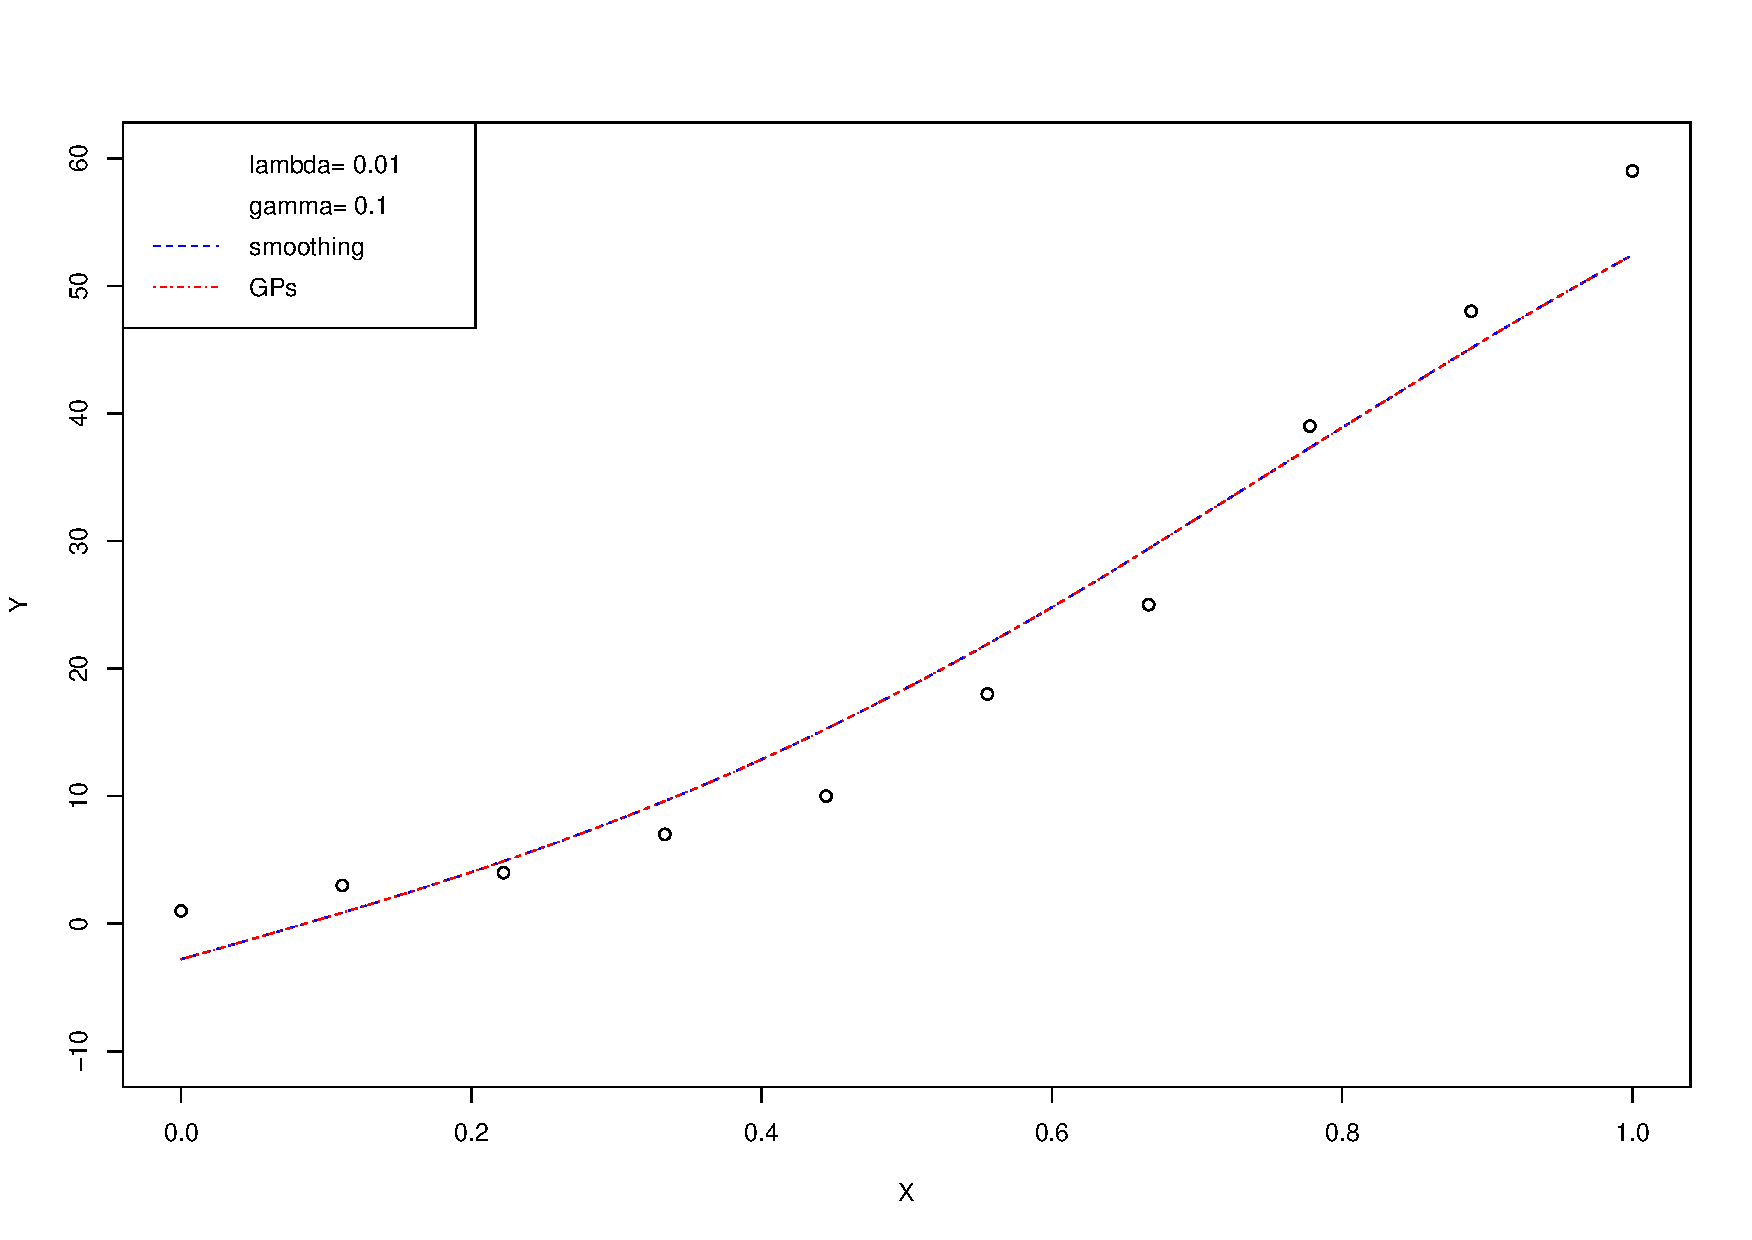
\includegraphics[width=8.5cm,height=6.5cm]{Chapters/2.TractorSplineTheory/plot/simu01} \\[\abovecaptionskip]
		\small (a) 
	\end{tabular}
	%    \vspace{\floatsep}
	\begin{tabular}{c}
		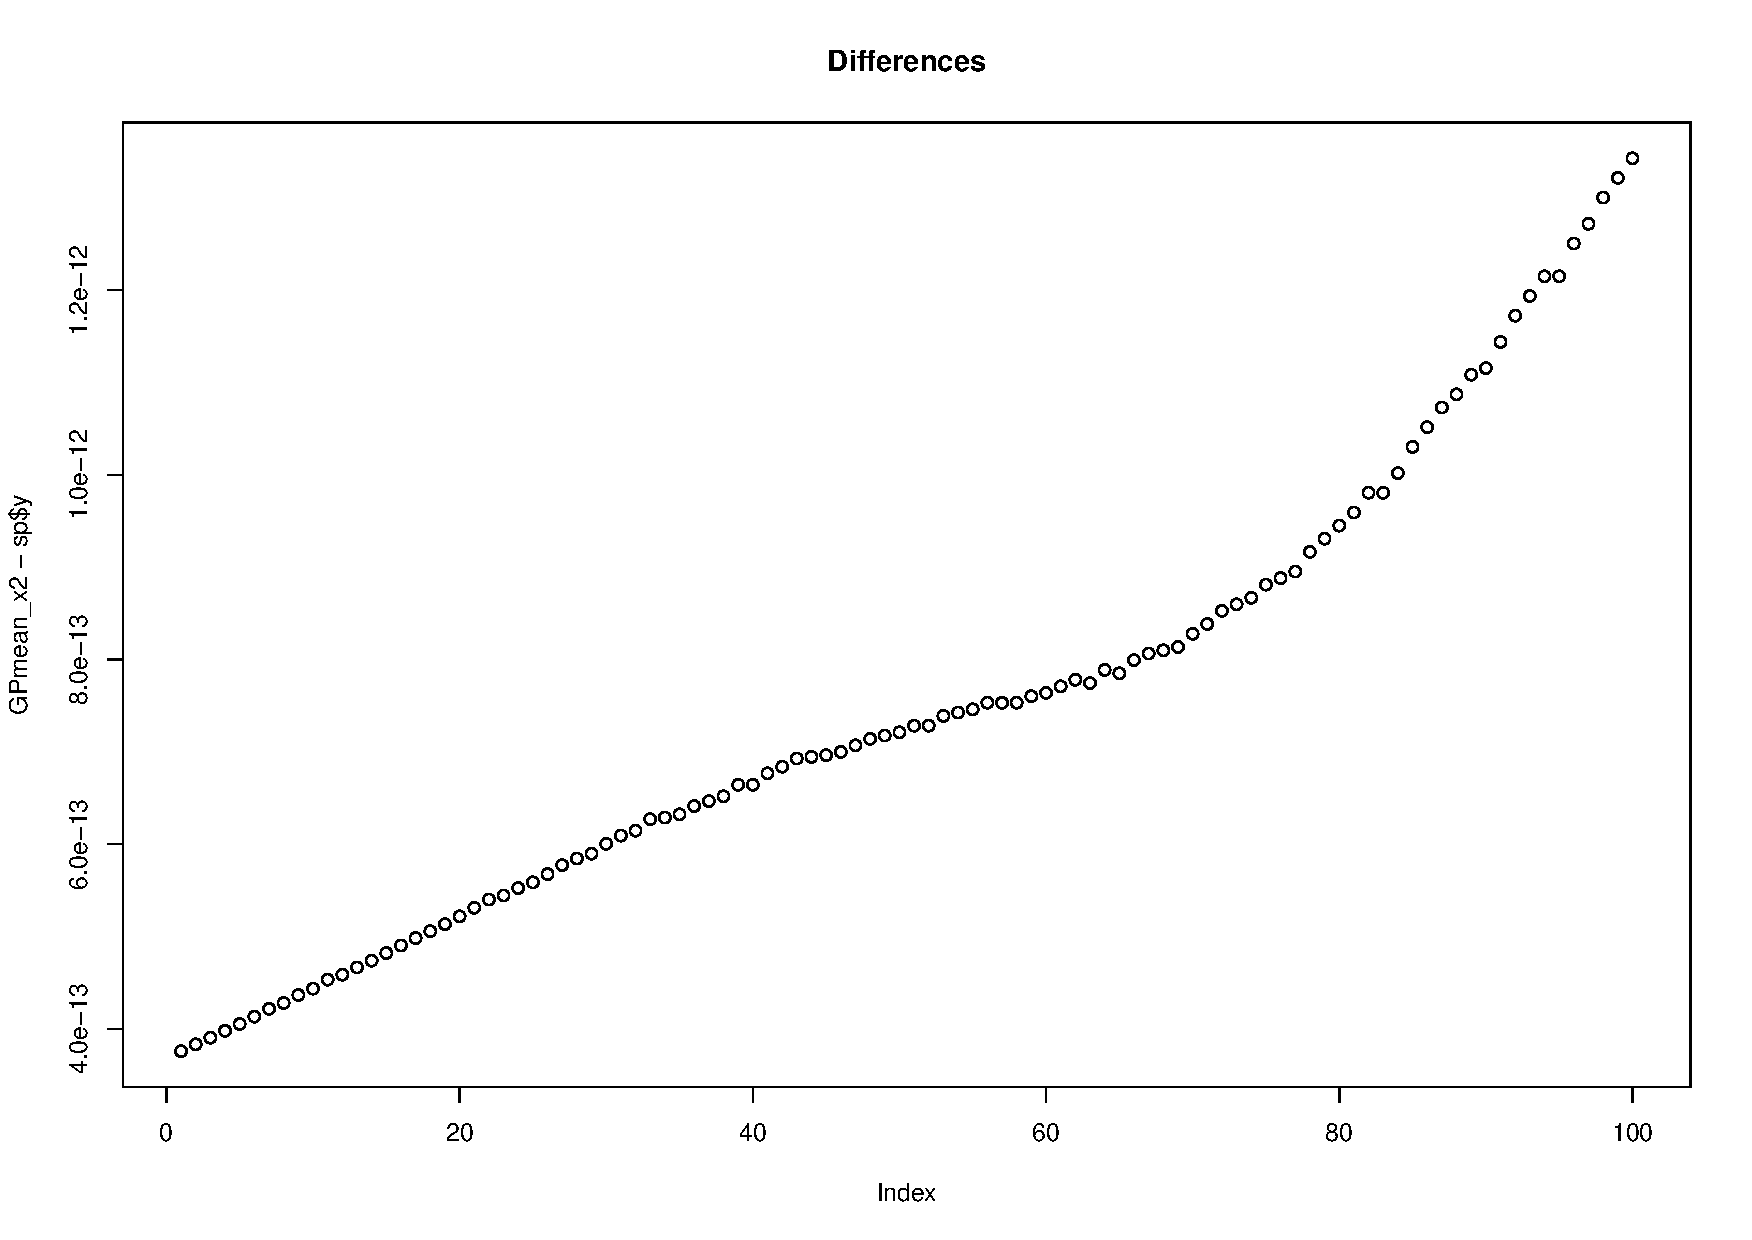
\includegraphics[width=8.5cm,height=6.5cm]{Chapters/2.TractorSplineTheory/plot/simu02} \\[\abovecaptionskip]
		\small (b) 
	\end{tabular}
	\caption{(a) Comparing two methods under the same parameters $\lambda=0.01$ and $\gamma=0.1$. In this graph, the blue line is reconstruction from tractor spline, the red line is the mean of Gaussian Process, which is the posterior $\mathbb{E}(\eta(x) | \mathbf{Y}, \mathbf{V})$. (b) The differences between two methods under the same parameters.}
\end{figure}

